\documentclass[times, utf8, zavrsni]{fer}
\setcounter{secnumdepth}{3}
\setcounter{tocdepth}{3}
\usepackage{booktabs}
\usepackage{algcompatible}
\usepackage{algorithm}
\usepackage{array}
\usepackage{subfigure}

\begin{document}

% TODO: Navedite broj rada.
\thesisnumber{000}

\title{Izrada rasporeda laboratorijskih vježbi uporabom genetskog algoritma}

\author{Filip Pankretić}

\maketitle

\izvornik

\zahvala{Zahvaljujem svojoj obitelji na svoj pružanoj podršci. Hvala im što su vjerovali u mene i bodrili me na mom putu.}

\tableofcontents
\listoffigures

\chapter{Uvod}

Izrada rasporeda problem je koji je prisutan svakodnevno, kako u obrazovnim institucijama poput škola, fakulteta, učilišta tako i u raspoređivanju satnice u industriji. Svaki raspored ima eksponencijalan broj konfiguracija i rješenje problema jednostavno nije izvedivo iscrpnim pretraživanjem kombinacija grubom silom.

Problem koji će se obrađivati u ovom radu podskup je tog problema, potrebno je generirati raspored laboratorijskih vježbi za 831 studenta u 37 grupa laboratorijskih vježbi bez preklapanja u njihovim rasporedima.

Cilj ovog rada je opisati rad metaheuristika, konkretno generacijskog genetskog algoritma koji pretražuje prostor stanja simuliranjem procesa evolucije. Potrebno je pomoću eksperimentalnih rezultata pronaći najbolju konfiguraciju algoritma koji će u konačnosti generirati kvalitetan raspored iskoristiv za neometano izvođenje nastave.

\chapter{Problem raspoređivanja studenata u grupe}

U obrazovnim institucijama dva najčešća problema slaganja rasporeda su dodjela grupa studentima i dodjela termina ispita. Raspored se smatra poželjnim ako profesor nema istovremeno dva predavanja, dva predmeta se istovremeno ne drže u istoj učionici, studenti nemaju više predavanja istovremeno i zadovoljena su sva stroga i što više blagih ograničenja \citep{ganguli2017study}.

Za većinu problema raspoređivanja pokazano je da su NP-teški\footnote{Ne postoji algoritam u polinomijalnom vremenu.} i da ne mogu biti riješeni u polinomnom vremenu koristeći deterministički algoritam. To vrijedi zbog kombinatorne eksplozije do koje dolazi zbog velikog broja, ograničenja, zahtjeva i velikog broja studenata, predmeta, nastavnika i slično.

Prilikom izrade rasporeda potrebno je paziti na dvije vrste ograničenja: \emph{stroga ograničenja} \engl{hard constraints} i \emph{blaga ograničenja} \engl{soft contraints}.

\section{Stroga ograničenja}

Stroga ograničenja odnose se na probleme koji su fizički nemogući. Poput toga da je profesor ili student na dva ili više mjesta istovremeno \citep{herath2017genetic}. Student mora imati dodijeljen samo jedan termin vježbi, a taj termin vježbi ne smije se preklapati s drugim terminima. Profesori koji održavaju vježbe ne smiju istovremeno održavati dva ili više termina, ali mogu imati dodijeljeno više termina u istom danu. U jednoj učionici istovremeno se ne može nalaziti više od jedne grupe studenata. Dodatne probleme mogu zadavati kapaciteti učionica, prilagođenost studentima s posebnim potrebama i slično.

\section{Blaga ograničenja}
Blaga ograničenja su ona koja se smatraju poželjnima, npr: jutarnji termini, želje profesora za određenim predavaonama, termini predavanja slijedno bez višesatnih pauza između. Često se stroga ograničenja zbog specifičnih situacija mogu tretirati kao blaga. Na primjer, kod predmeta s neobaveznom prisutnošću broj studenata smanji  se nakon prvih nekoliko predavanja pa kršenjem maksimalnog kapaciteta ne nastaje veliki problem.

\chapter{Genetski algoritam}
\textbf{Evolucijsko računanje} je grana umjetne inteligencije koja se, najvećim dijelom, bavi rješavanjem optimizacijskih problema \citep{cupic-disertacija}. Evolucijsko računanje je familija metaheuristika\footnote{Skup algoritamskih koncepta primjenjivih na širok spektar problema} inspiriranih prirodnim procesima i biološkom evolucijom. Dijeli se na  3 grane: \emph{evolucijske algoritme}, \emph{algoritme rojeva} i \emph{ostalo}. 

\begin{figure}[htb]
\centering
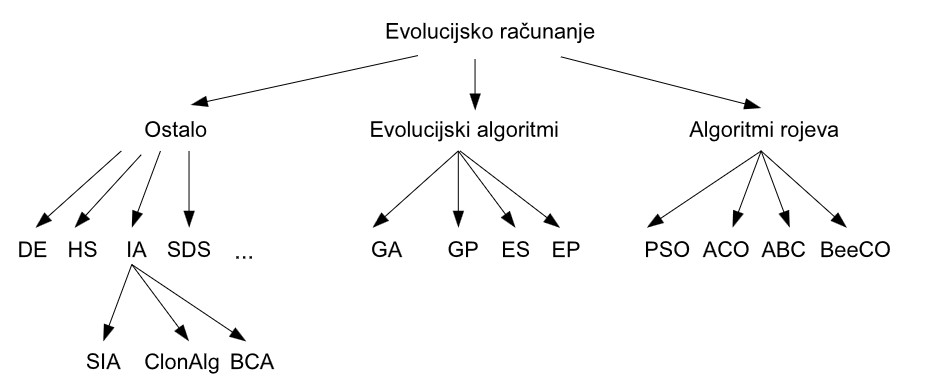
\includegraphics[width=15cm]{images/evolucijske_grane.png}
\caption{Podjela evolucijskog računanja na glavne grane uz odabrane algoritme \citep{cupic-disertacija}.}
\label{fig:evolucijske_grane}
\end{figure}

Evolucijski algoritmi inspirirani su Darwinovom teorijom o postanku vrsta koja se temelji na 5 pretpostavka:

\begin{enumerate}
	\item potomaka uvijek ima više nego je potrebno
	\item veličina populacije je prillbižno stalna
	\item količina hrane je ograničena
	\item kod vrsta koje se seksualno razmnožavaju, nema identičnih jedinki već postoje varijacije
	\item najveći dio varijacija prenosi se nasljeđem.
\end{enumerate}

	\textbf{Genetski algoritam} jedan je od evolucijskih algoritama stvorenih za rješavanje optimizacijskih problema, a koji izravno utjelovljuje navedene postavke \citep{cupic-skripta}.  Klasični evolucijski algoritam sadrži slijedeće dijelove:
	
\begin{itemize}
	\item \textbf{Populacija} - podskup svih mogućih rješenja danog problema.
	\item \textbf{Jedinka} - jedno od rješenja u populaciji.
	\item \textbf{Funkcija dobrote} - numerička oznaka kvalitete neke jedinke.
	\item \textbf{Operator odabira roditelja} - operator odabira roditelja za daljnje križanje.
	\item \textbf{Operator križanja} - operator kombiniranja dviju jedinki kako bi se generirao jedan ili dva potomka.
	\item \textbf{Operator mutacija} - operator koji se koristi kako bi se održala raznolikost jedinki.
\end{itemize}

Sekvencijski\footnote{Rade u jednodretvenim sustavima} genetski algoritam može se podijeliti na dvije tipične izvedbe: \emph{eliminacijski genetski algoritam} \engl{steady-state genetic algorithm} i \emph{generacijski genetski algoritam} \engl{generational genetic algorithm} \citep{cupic-disertacija}. Kako se \emph{generacijski genetski algoritam} koristi za rješenje zadanog problema, njegov pseudokod je dan u nastavku:

\begin{algorithm}
\caption{Generacijski genetski algoritam}
\label{algo:generational-algo}
\begin{algorithmic}
\STATE{populacija := new jednika[N]}
\STATE{dobrota := new ocjena[N]}
\FOR{i := 0; i < N; i++}
\STATE{dobrota[i] := ocijeni(populacija[i])}
\ENDFOR
\WHILE{nije kraj}
\STATE{pom\_populacija := new jednika[N]}
\STATE{pom\_dobrota := new ocjena[N]}
\FOR{i := 0; i < N; i++}
\STATE{roditelj1 := odabirRoditelja(populacija)}
\STATE{roditelj2 := odabirRoditelja(populacija)}
\STATE{dijete := križaj(roditelj1, roditelj2)}
\ENDFOR
\algstore{generational-algo}
\end{algorithmic}
\end{algorithm}

\newpage

\begin{algorithm}
\begin{algorithmic}
\algrestore{generational-algo}
\STATE{populacija := pom\_populacija}
\STATE{dobrota := pom\_dobrota}
\ENDWHILE
\end{algorithmic}
\end{algorithm}

Kod generacijskog genetskog algoritma eventualno dobro dijete ne može se odmah iskoristiti; ono mora pričekati dok se ne završi čitava generacija.

Generacijski algoritam može taokođer biti elitistički\footnote{Svojstvo algoritma da sadrži najbolju jedinku}. Za razliku od neelitističkih inačica, kroz evoluciju graf jedinki bit će nazubljen te najbolja jedinka nove generacije ne mora biti bolja od prethodne \citep{cupic-skripta}.

\chapter{Dodjela termina laboratorijskih vježbi}
\label{ch:glavni}

Problem dodjele termina laboratorijskih vježbi znatno je lakši od izrade cjelovitog rasporeda. Nasuprot originalnog problema izrade cjelovitog rasporeda, sad postoji već prethodno izrađen raspored i isti je potrebno popuniti dodatnim terminima laboratorijskih vježbi. Također, nije potrebno uzeti u obzir cijeli raspored već samo jedan tjedan u semestru, što znatno olakšava problem i sami pristup problemu. Nadalje, nije potrebno pratiti niti sljedeće stavke: željeni termini profesora ili asistenata, profesori ili asistenti dodijeljeni terminu, održavaju li se dva ili više termina istovremeno itd. Općenito je potrebno paziti na navedena ograničenja, ali trenutno ne spadaju u opseg ovog rada.

\section{Reprezentacija rasporeda u obliku jedinke}

Svaki generirani raspored (također istoznačno: jedinka) potrebno je ispravno prikazati u memoriji. Ovisno o zapisu koji se koristi, problem se može znatno olakšati ili otežati. Osim zapisa same jedinke, program prima niz datoteka potrebnih za rad algoritma: popis studenata, popis dostupnih termina laboratorijskih vježbi, maksimalan i minimalan broj studenata po terminu te prethodna zauzetost studenata.

Prvo je potrebno definirati univerzalne podatke koji se koriste neovisno o zapisu samog rasporeda. Zapis termina laboratorijskih vježbi dan je formatu:

\emph{šifra\_termina;kapacitet;datum;vrijeme\_početaka;vrijeme\_kraja;učiona}, gdje je dodatno \emph{kapacitet} u formatu: \emph{makimalan\_kapacitet/minimalan\_kapacitet}. Svaki zapis spremamo u četiri odvojena niza: niz s cijelovitim zapisom, niz s početkom termina, niz s krajem termina i niz s datumom termina. Nadalje se termini referenciraju indeksom na kojem su raspoređeni.

Slijedi prikaz termina studenata. Moguće je da se u tablici zauzetosti studenata nalaze studenti kojima nije potrebno dodijeliti termin. Stoga se za prikaz rasporeda koristi tablica raspršenog adresiranja\footnote{Struktura podataka koja u pretincima adresiranim nekim ključem sadrži određeni tip podatka.} koja kao ključ prima JMBAG\footnote{Jedinstveni matični broj akademskog građanina} studenta, kao vrijednost sadrži još jednu tablicu koja sada prima kao ključ datum termina, a kao vrijednost ima strukturu podataka vektor\footnote{Struktura podataka koji automatski alocira i dealocira memoriju, a ponaša se kao niz} s popisom prethodnih termina. Slijedni termini se spajaju u jedan zajednički termin kako bi se kasnije ubrzala provjera kolizija. Kolizije već prethodno dodijeljenih termina prilikom učitavanja podataka ne provjeravaju se.

\begin{figure}[htb]
\centering
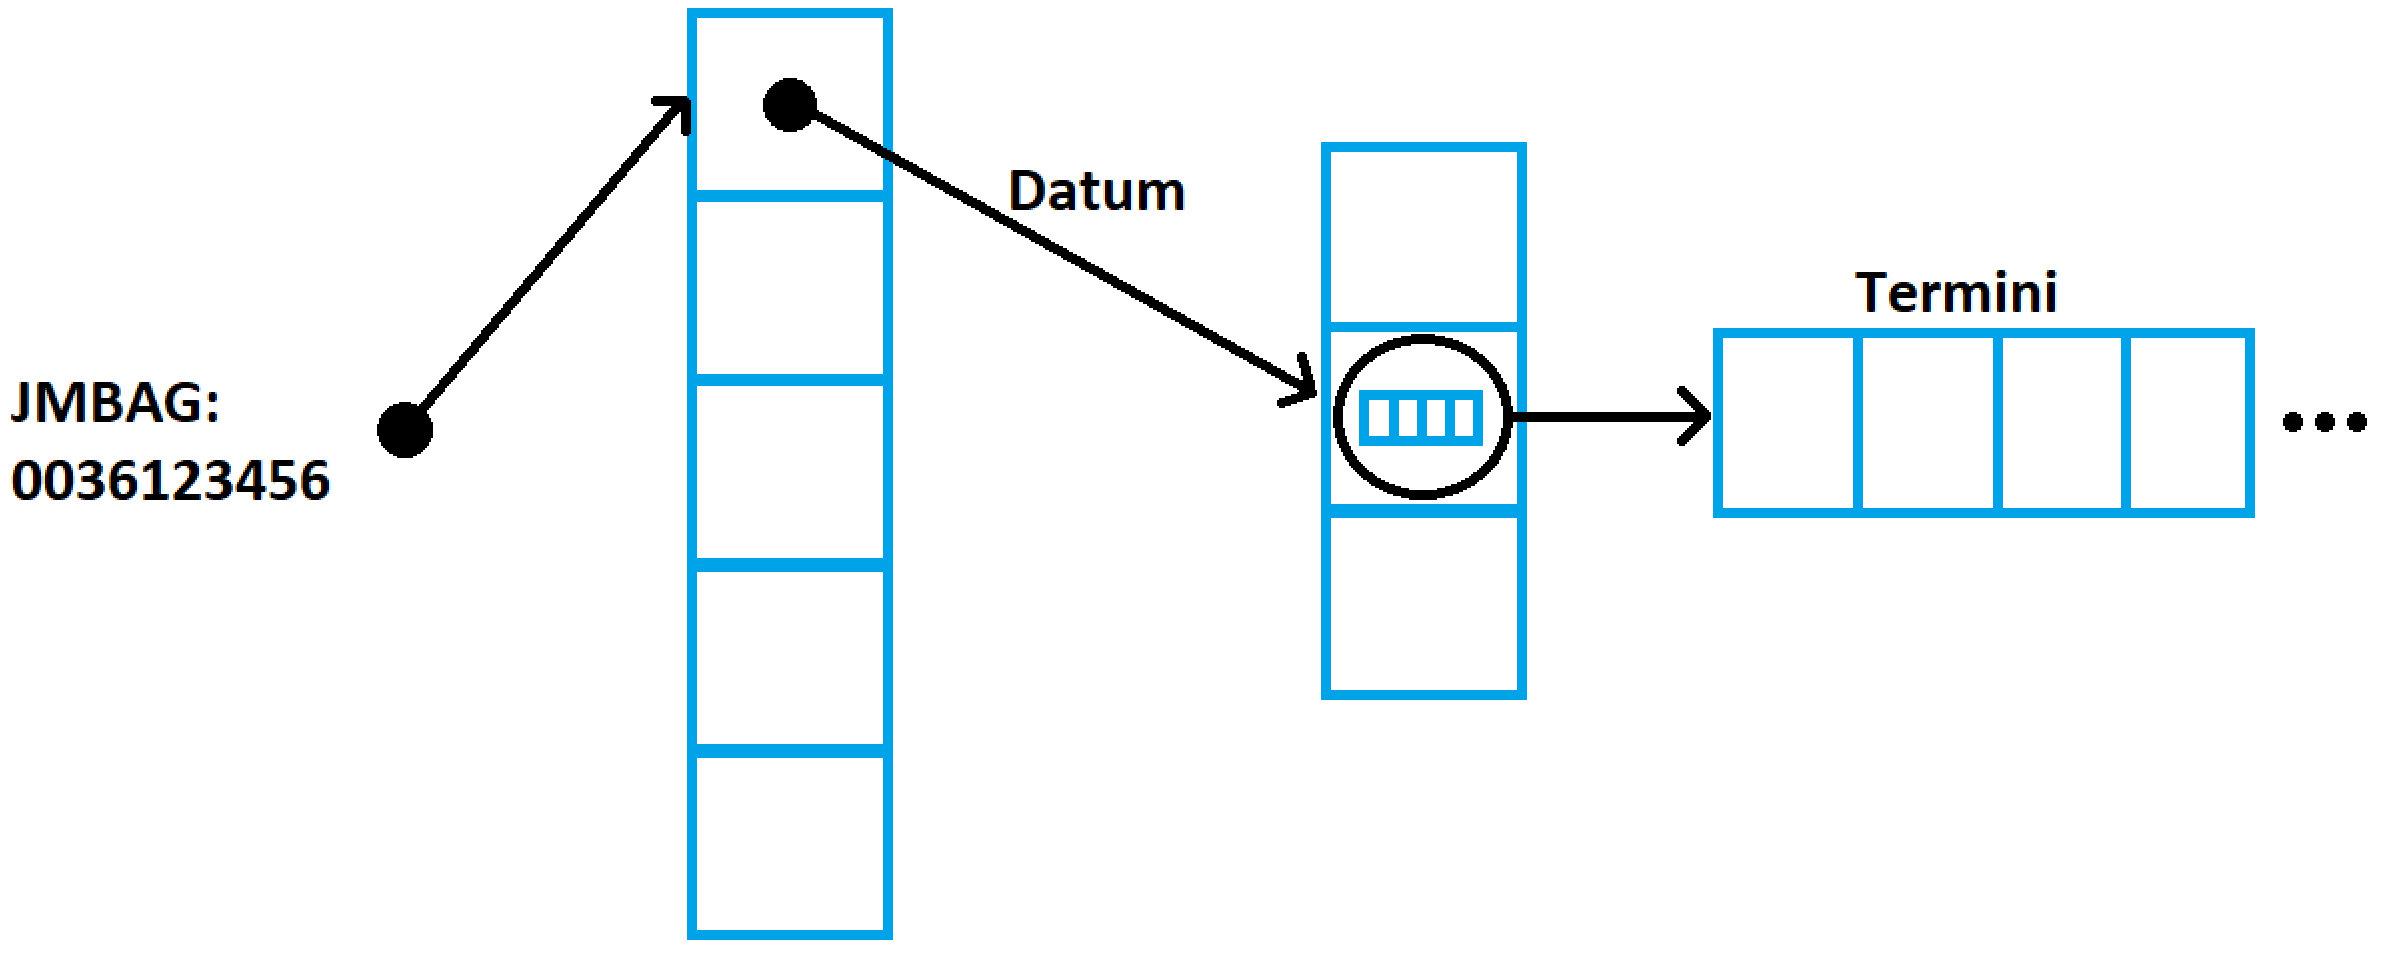
\includegraphics[width=15cm]{images/prikaz_termina.png}
\caption{Prikaz zapisa nastavnih obveza studenata u memoriji.}
\label{fig:prikaz_termina}
\end{figure}

Popis studenata kojima je potrebno dodijeliti termin mogu sadržavati termin koji ne postoji u tablici prethodno dodijeljenih termina U tom slučaju pretpostavlja se da student u tom tjednu nema ostalih nastavnih obveza. Studenti se prikazuju kao niz JMBAG-ova kojemu se kasnije pristupa preko indeksa pojedinog elemenata.

Dva načina zapisa rasporeda koja će biti obrađena su \emph{niz termina s listom studenata} i \emph{niz studenata s dodijeljenim terminom}.

\subsection{Niz termina s listom studenata}

Prvi način zapisa je niz termina gdje svaki element tog niza sadrži vektor sa studentima kojima je dodijeljen taj termin.

\begin{figure}[htb]
\centering
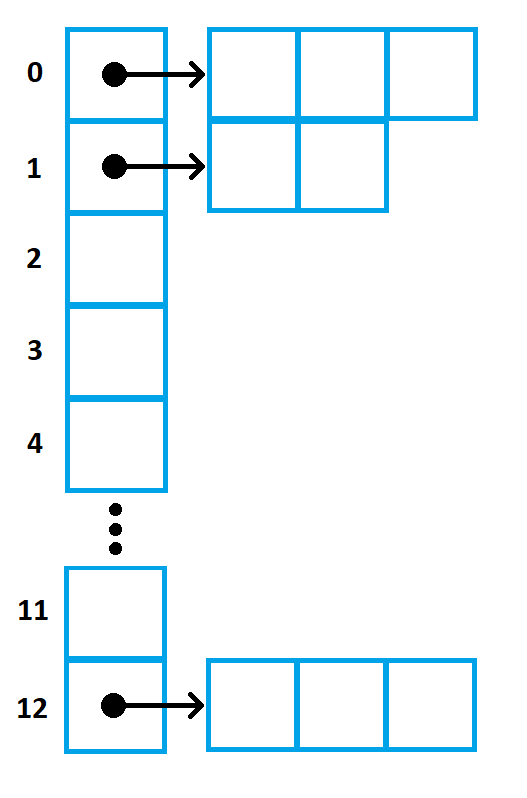
\includegraphics[width=7cm]{images/prikaz_jednike_1.png}
\caption{Prikaz niza termina s listom studenata u memoriji.}
\label{fig:prikaz_jednike_1}
\end{figure}

Prednosti ovog zapisa su lakši ispis podataka jer svaki termin odmah sadrži popis studenata i jednostavnija provjera zauzetog kapaciteta nekog termina. Prednosti je vrlo malo, dok mana ima puno više.

Neki od nedostataka su da je potrebno paziti da je svaki student dodijeljen samo jednom terminu, teže je implementirati operatore mutacije i operator križanja jer jedinka ima dvije osi od kojih je jedna varijabla. Također je zbog toga otežan izračun preklapanja. Dodatno, ovaj prikaz je i memorijski i vremenski zahtjevan zbog korištenja dodatnih struktura podataka.

\subsection{Niz studenata s dodijeljenim terminom}

Drugi način prikaza je niz gdje indeks svakog elementa predstavlja jednog studenta, a element je indeks dodijeljenog termina.

Ovaj način pruža jednodimenzionalni niz što znatno olakšava definiranje operatora križanja i mutacije. Kako svaki student predstavlja jedan element niza, odmah je riješeno tvrdo ograničenje da student može pristupiti samo jednom terminu laboratorijskih vježbi. Lakše je izračunati pojedina preklapanja jer je za svakog studenta jednostavno pronaći dodijeljeni termin. Memorijski i vremenski je efikasniji od prvog načina zbog jednostavnije strukture.

Otežan je izračun zauzetog broja mjesta po terminu i ispis podataka. Za provjeru zauzeća potrebno je jednom proći  kroz cijeli niz kako bi se za svaki termin prebrojala zauzeta mjesta, a za ispis rasporeda potrebno je za svaki termin proći kroz cijeli niz i ispisati studenta kako se naiđe na njega ili je potrebno u zasebnoj strukturu držati popis studenata slično kao prvi zapis. Kako se raspored ispisuje samo povremeno, to ne predstavlja problem.

\begin{figure}[htb]
\centering
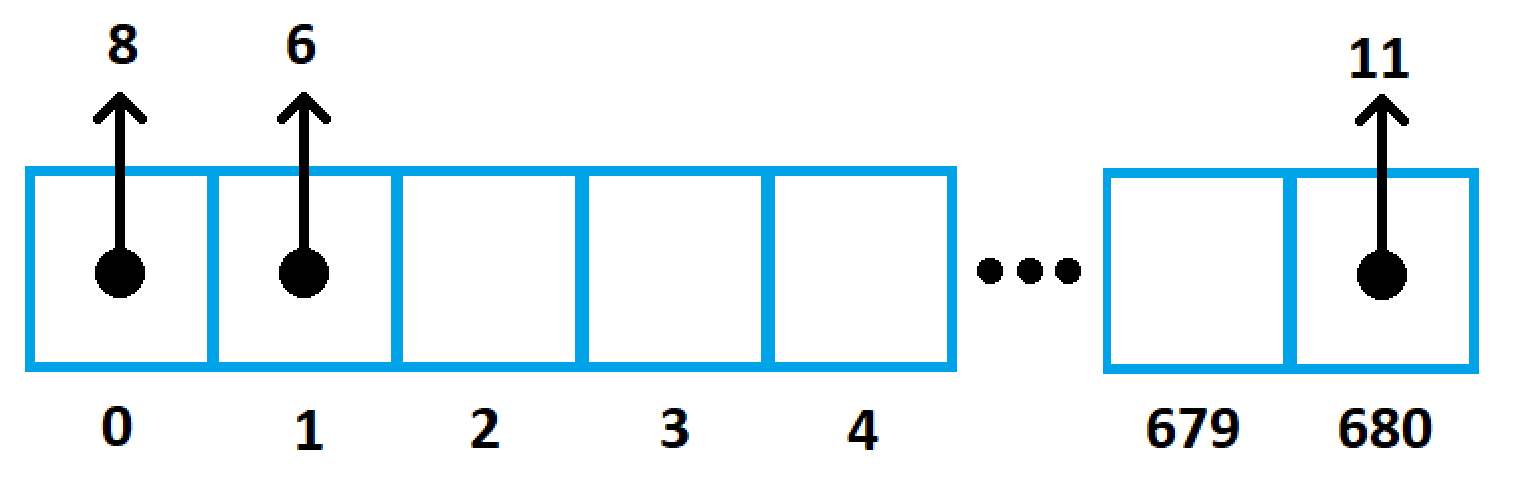
\includegraphics[width=13cm]{images/prikaz_jednike_2.png}
\caption{Prikaz niza termina s listom studenata u memoriji.}
\label{fig:prikaz_jednike_2}
\end{figure}

Zbog velikog broja prednosti druge strukture naspram prve, ta struktura odabrana je za prikaz rasporeda.

\section{Ocjena rasporeda}

Ocjena rasporeda rezultat je funkcije dobrote \engl{fitness}. Točnije, to je numerička oznaka koja se koristi za ocjenu kvalitete rasporeda. Ukupna ocjena nekog rasporeda jednaka je sumi funkcija dobrote za svakog studenta iz nekog rasporeda.

\begin{equation}
\sum_{i=0}^{n} dobrota(student[i])
\label{eq:dobrota}
\end{equation}

\subsection{Dobrota i kazna}

Osim dobrote, raspored može koristiti i kaznu \engl{punishment}. Kazna je mjera koliko je neki raspored loš. Ponekad je za problem lakše definirati ukupnu kaznu, nego ukupnu dobrotu. U praksi se pokušava ili minimizirati kazna ili maksimizirati dobrota. Kazna, kao i dobrota, zapravo je heuristika koja aproskimira koliko je daleko, odnosno blizu, dobiveno rješenje od cilja, tj.\ najboljeg rješenja.

U sklopu ovog rada, najbitnije je svojstvo rasporeda da nema preklapanja, stoga će bolji raspored biti onaj koji ima manje preklapanja, a potom onaj koji ima bolju ocjenu.

Prilikom izračuna ocjene rasporeda, sljedeća svojstva uzeta su kao pretpostavke:

\begin{itemize}
	\item studenti preferiraju imati vježbe u istom danu kad već imaju nastavne aktivnosti
	\item bolji je termin koji stvara manju rupu do najbliže nastave aktivnosti nego onaj koji stvara veću
	\item broj nastalih pauza u rasporedu nije bitan i 
	\item bolji je termin koji je slijedno s nastavnim aktivnostima bez pauze neovisno o opterećenju taj dan.
\end{itemize}

\subsubsection{Dobrota}

Kad bi raspored koristio dobrotu za svoju ocjenu, neke od heuristika koje bi se mogle koristiti su broj studenata koji nemaju preklapanje i broj studenata kojima je dodijeljen termin slijedno s ostalim nastavnim aktivnostima.

Teško je definirati kvalitetnu funkciju dobrote za raspored jer je vrlo malo svojstva kojima se može dodijeliti smislena numerička vrijednost. Čak i ako se uspiju pronaći smislene karakteristike za funkciju dobrote, teško je namjestiti vrijednosti tako da algoritam preferira sva svojstva istovremeno.

Na primjer, ako se za svakog studenta bez preklapanja funkcija dobrote poveća za 10, a za svaki slijedni raspored se poveća za 5, algoritam će vrlo vjerojatno preferirati studente koji nemaju preklapanja, a neće preferirati da studenti imaju slijedna predavanja. Opet, može se dogoditi da algoritam sve studente stavi u nekoliko termina gdje svi studenti imaju slijedna predavanja, ali s puno preklapanja i puno prekršenih ograničenja.

\subsubsection{Kazna}

Rasporedi sati esencijalno imaju jako puno ograničenja koja ne smiju biti prekršena ili smiju, ali do neke granice. Stoga, lakše je implementirati funkciju kazne rasporeda. Za kaznu, isto kao i za dobrotu, vrijedi da ako se postavi prevelika kazna za bilo koje svojstvo, vjerojatno je da će dominirati rasporedi koji imaju minimiziranu kaznu s tim svojstvom.

Naime, kako je cilj pronaći raspored koji nema preklapanja, to ne predstavalja preveliki problem, ali ako se koristi kazna umjesto dobrote za ocjenu algoritma, dostupan je puno veći broj heuristika koje mogu potencijalno pronaći kvalitetniji raspored.

Neke od dostupnih heuristika su: broj preklapanja, broj pauza, vrijeme preklapanja, koliko su prekršeni zahtjevi kapaciteta nekog termina i vremenski period najmanje pauze nastale nakon dodavanja termina.

\subsubsection{Kazna s kombinacijom dobrote}
\label{sec:kombinacija}

Kao najbolja opcija ipak se pokazala kazna s kombinacijom dobrote. Osim heuristika kazne, uvodi se mali broj heuristika koje rasporedu daju nagradu, to jest smanjuju kaznu za iznos pomnožen malim koeficijentom ako su zadovoljena neka dobra svojstva u rasporedu. Kada bi nagrada bila velika, onda bi algoritam zapravo pokušavao maksimizirati nagradu umjesto da minimizira kaznu.

\subsection{Ograničenje broja studenata}

Kod izračuna cijene prilikom kršenja maksimalnog ili minimalnog kapaciteta koriste se sljedeće pretpostavke:

\begin{itemize}
	\item minimalni broj studenata u terminu je uvijek 15
	\item maksimalan broj studenata u terminu je uvijek 16
	\item gore je kada broj studenata premaši maksimalan kapacitet, nego kad je broj studenta manji od minimuma.
\end{itemize}

Nakon što je dostupna informacija o broju studenata za svaki termin, dodjeljuje se kazna ovisno o prekršenim ograničenjima. Kazna za termine kojima je dodijeljen veći broj studenata od maksimalnog jednaka je razlici broja dodijeljenih studenata i maksimalnog broja studenata za taj termin pomnožena s nekim koeficijentom.

\begin{equation}
(brojStudenata - 16) \cdot koeficijentZaViseStudenata
\label{eq:max-studenta}
\end{equation}

Istovjetno, termini kojima je dodijeljen manji broj studenata od minimalnog doprinose kaznom jednakom razlici minimalnog broja studenata i dodijeljenog broja studenata pomnoženom s nekim koeficijentom.

\begin{equation}
(15 - brojStudenata) \cdot koeficijentZaManjeStudenata
\label{eq:min-studenta}
\end{equation}

Koeficijent za manji i veći broj studenata nisu jednaki, što se temelji na trećoj zadanoj pretpostavci. Nastavniku je očigledno jednostavnije ispitati manji broj studenata od minimuma, nego veći od maksimuma, zato je koeficijent za manje studenata manji od onog za više. Dobro svojstvo za ta dva koeficijenta je da njihova razlika ne bude prevelika. Jer, ako bi koeficijent za manji broj studenata bio premali, onda bi algoritam mogao dominirati rasporedima koji nemaju popunjena sva mjesta u učionicama, a isto vrijedi i obratno.

\subsection{Izračun preklapanja}

Student može imati preklapanja u rasporedu prije nego li mu je dodijeljen termin laboratorijskih vježbi. Kod takvih situacija računaju se zasebno kolizije dodijeljenog termina sa svakim prethodnim terminom zasebno, tako da teoretski jedan student može proizvesti više od jedne kolizije. Kazna se dodjeljuje svakoj od tih kolizija kako bi se čak i u slučaju kolizija što prije odbacio raspored gdje pojedinim studentima gotovo pa nije moguće pristupiti terminu laboratorijskih vježbi.

Preklapanje dvaju termina lako se može provjeriti formulom:

\begin{equation}
max(t1, T1) - min(t0, T0) < (t1 - t0) + (T1  - T0)
\label{eq:preklapanje}
\end{equation}

\emph{T0} i \emph{T1} predstavljaju redom početak i kraj dodijeljenog termina, a \emph{t0} i \emph{t1} redom početak i kraj nekog od termina ostalih nastavnih obveza. \emph{max(t1, T1) - min(t0, T0)} predstavlja interval na kojem se nalaze termini koji se trenutno uspoređuju i ako je taj interval manji od zbroja duljina zasebnih intervala, onda postoji preklapanje.

\begin{figure}[htb]
\centering
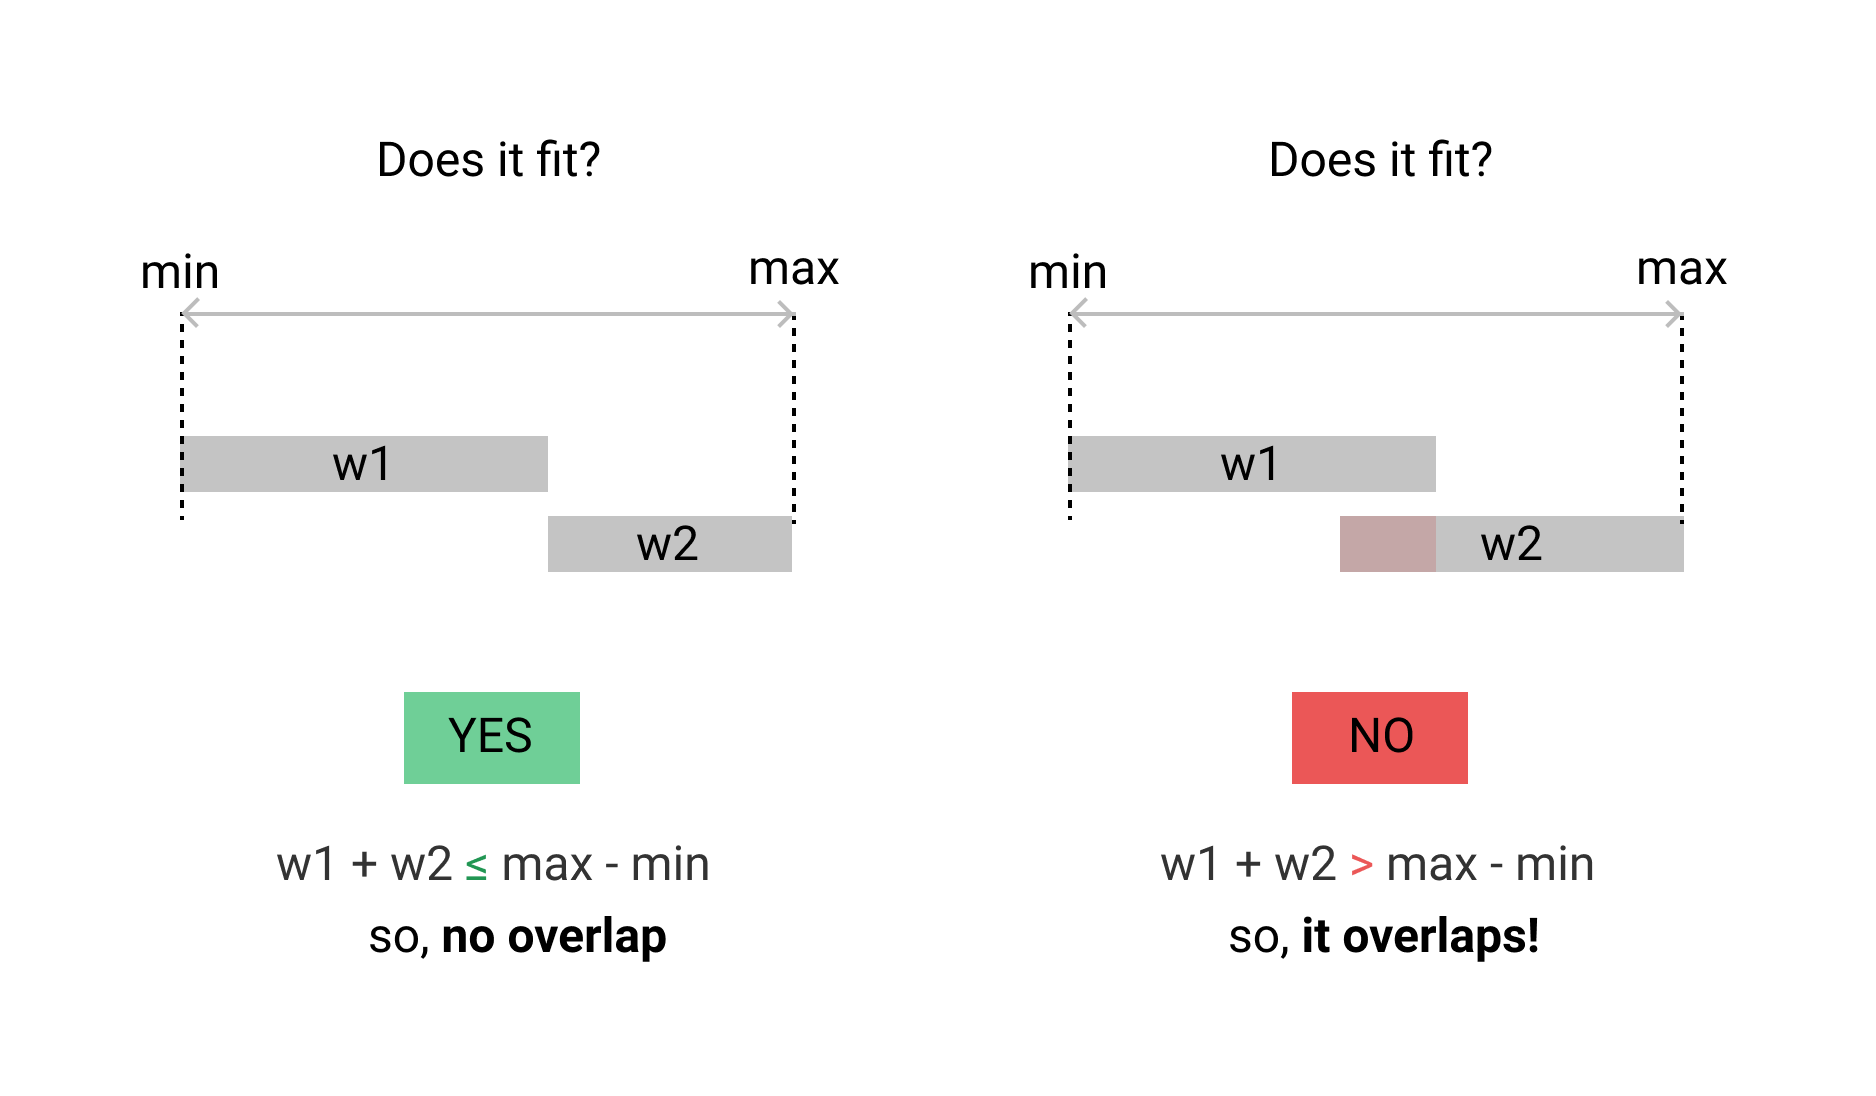
\includegraphics[width=15cm]{images/preklapanja.png}
\caption{Provjera preklapanja dvaju termina.}
\label{fig:preklapanja}
\end{figure}

Najvažnije svojstvo rasporeda je da ima minimalni broj preklapanja, zato se umnožak preklapanja množi s koeficijentom koji je veći od ostalih. Razlog tome je kako bi se što prije pronašao raspored koji ima minimalan broj preklapanja i onda se krenulo u dodatno poboljšanje ostalih svojstva rasporeda.

\subsection{Slijedni termini}

Kao što je spomenuto u poglavlju \ref{sec:kombinacija}, zbog nekih poželjnih svojstava rasporedu se može dodijeliti nagrada. Nagrada je implementirana tako da ukupnu kaznu rasporeda smanji za neku brojčanu konstantu. Manje konstante osiguravaju, pogotovo ako je implementirano više nagrada, da se ne preferiraju rasporedi s više nagrada i manje prekršenih ograničenja. 

Jedno od tih svojstva je slijedno održavanje termina. Slijednost se provjerava samo ako se navedeni termin ne preklapa s niti jednim ostalim terminom. Za provjeru slijednosti može se koristiti formula \ref{eq:preklapanje}, ali tako da se znak nejednakosti promijeni u znak jednakosti.

\begin{equation}
max(t1, T1) - min(t0, T0) = (t1 - t0) + (T1  - T0)
\label{eq:slijednost-long}
\end{equation}

Ali, zbog toga što provjera slijednosti ponovo uspoređuje dobiveni termin sa svim ostalim terminima, poželjno je, ako je moguće, ubrzati provjeru. Zato se za provjeru preklapanja dvaju termina koristi sljedeća formula:

\begin{equation}
t0 = T1 \lor T0 = t1
\label{eq:slijednost-short}
\end{equation}

gdje \emph{T0, T1, t0} i \emph{t1} imaju isto značenje kao i formula \ref{eq:preklapanje}. Dovoljno je samo provjeriti počinje li ili završava dodijeljeni termin onda kada bilo koji drugi redom završava ili počinje.

\subsection{Pauza nastala nakon dodijeljenog termina}

Broj pauza u rasporedu nije bitan, već se za izračun kazne koristi samo minimalna udaljenost dodijeljenog termina do svih ostalih termina. Provjera pauza se ne vrši u slučaju da su već pronađena dva slijedna termina ili ako postoji kolizija. Za pronalazak najmanjeg perioda pauze u rasporedu koristi se sljedeća formula:

\begin{equation}
min(|T0 - t1|, |T1 - t0|)
\label{eq:min-rupa}
\end{equation}

\noindent
gdje \emph{T0, T1, t0} i \emph{t1} imaju isto značenje kao i formula \ref{eq:preklapanje}. Potom se kazna povećava za iznos izračunat formulom:

\begin{equation}
koeficijent \cdot najmanjiRazmak^2
\label{eq:min-rupa-kazna}
\end{equation}

Koeficijent služi za podešavanje doprinosa kazne. Prema pretpostavci bolji je raspored onaj koji nema pauze što znači da će rasporedi s većom pauzom biti gori, tj. imat će veću kaznu. Kako bi se ta pauza što više minimizirala, najmanji razmak se kvadrira kako bi se studentima dodijelili termini sa što manjim vremenskim razmakom.

\subsection{Termin dodijeljen u danu bez nastavnih obveza}

Temeljeno na prvoj pretpostavci izračuna ocjene rasporeda, studenti preferiraju termine laboratorijskih vježbi u istom danu kada imaju neku drugu nastavnu aktivnost, stoga ako student nema drugih nastavnih aktivnosti u danu održavanja laboratorijskih vježbi, dodjeljuje se kazna relativno velikog iznosa.

Provjera ima li student neke druge nastavne aktivnosti tog dana održava se na samom početku prije provjera preklapanja, slijednosti termina i pauze s najmanjim vremenskim razmakom. Ako je ta provjera istinita, onda se ostala svojstva ne provjeravaju.

\section{Elitizam}

\textbf{Elitizam} \engl{elitism} je svojstvo algoritma da uvijek sadržava najbolji raspored.

Odabir elitnog rasporeda vrši se tako da se prolazi kroz kazne svih jedinki i gleda se ima li raspored manji broj preklapanja od prethodnoga. U slučaju da ima, raspored na kojeg se naišlo bira se kao elitni, a u slučaju da je broj preklapanja jednak, onda se odabire onaj s manjom kaznom.

Kod elitističkih algoritama graf koji prikazuje kretanje funkcije kazne kroz evoluciju je monoton. Zbog načina odabira elitinog rasporeda, ovdje će to svojstvo monotonosti biti vidljivo oko 1000 iteracije kada broj preklapanja postane nula.

\begin{figure}[htb]
\centering
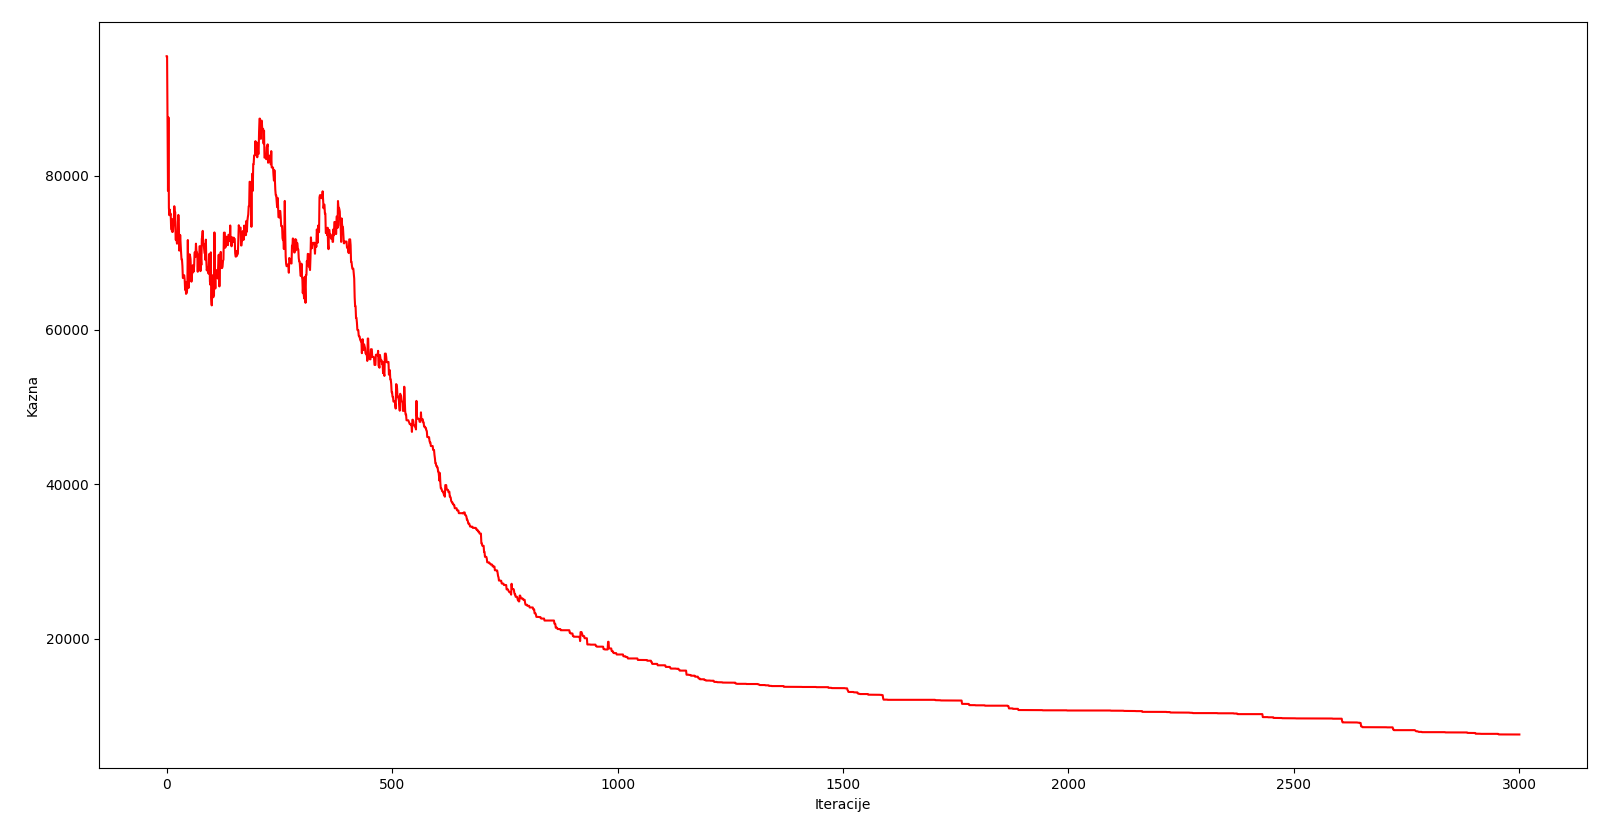
\includegraphics[width=14cm]{images/elitizam_da.png}
\caption{Generirani raspored s uključenim elitizmom.}
\label{fig:elitiziam_da}
\end{figure}

Kod algoritama koji nisu elitistički taj će graf biti nazubljen: prosječne vrijednosti funkcije kazne asimptotski će padati, ali je sasvim moguće da u nekon koraku algoritma kazna najbolje jedinke bude veća od kazne najbolje jedinke koju je algoritam imao u nekom prethodnom koraku \citep{cupic-skripta}.

\begin{figure}[htb]
\centering
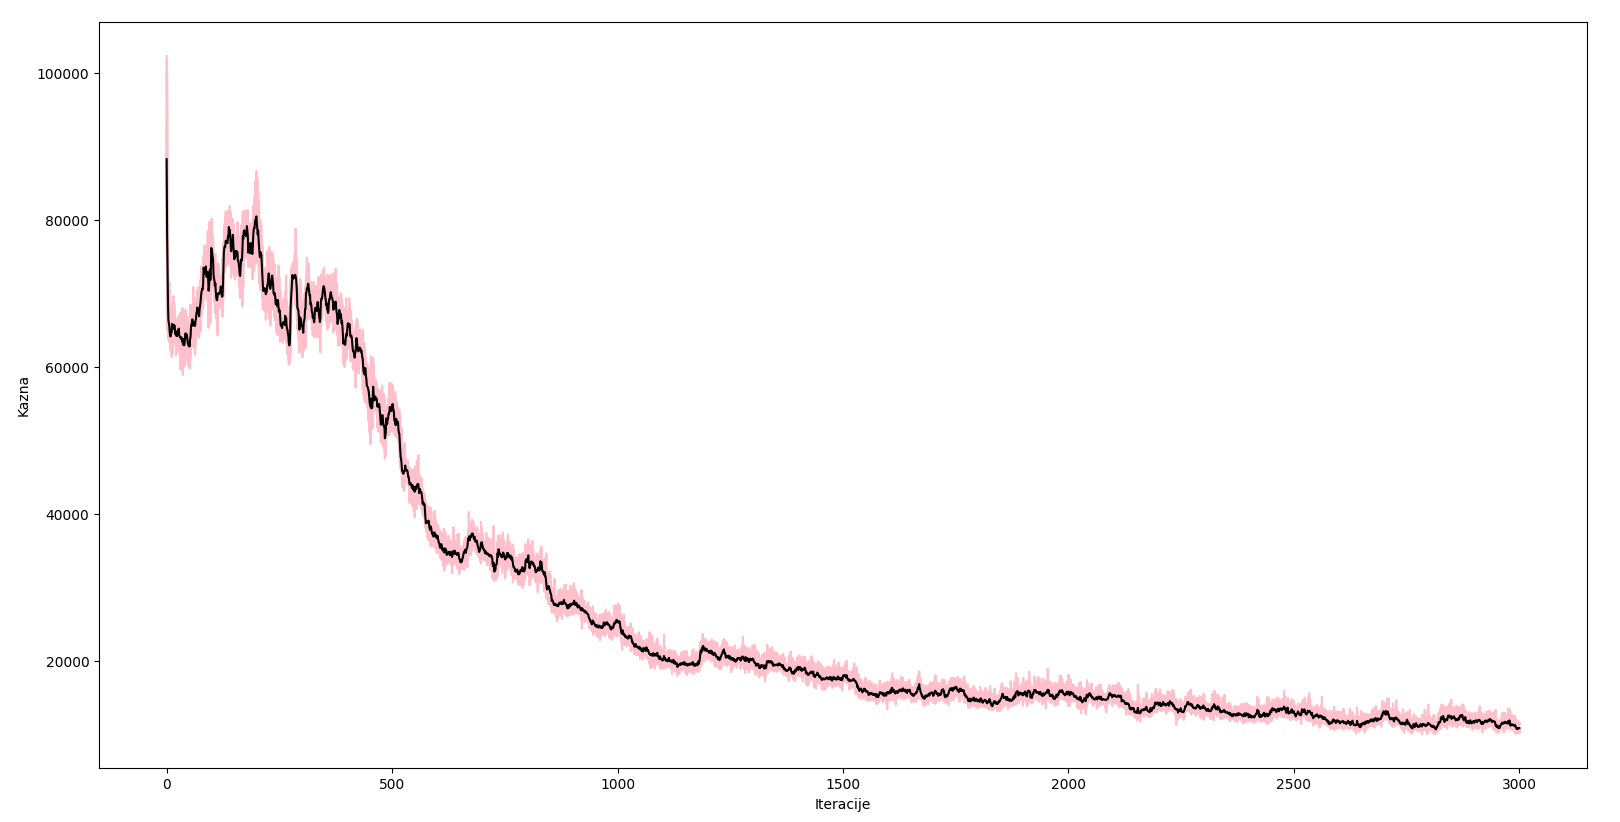
\includegraphics[width=14cm]{images/elitizam_ne.png}
\caption{Generirani rasporedi s isključenim elitizmom.}
\label{fig:elitiziam_ne}
\end{figure}

Prilikom izrade rasporeda, očuvanje elitnog rasporeda je pokazalo dobra svojstva poput brže konvergencije i manjeg raspršenja. A kod nekih postavka algoritma, jedino su s uključenim elitizmom rasporedi počeli konvergirati. To je zato što elitni raspored pruža algoritmu točku za koju se može držati kako bi se odupro divergenciji zbog raznih loših utjecaja na algoritam. Tako sada algoritam postaje striktno konvergentan.

\section{Odabir roditelja}

Kod odabira roditelja važno je da oba roditelja budu različita kako bi se održala raznolikost rasporeda. Kada bi oba odabrana roditelja bila jednaka, raspored nastao operatorom križanja bio bi jednak roditeljima, a to nije poželjno svojstvo genetskog algoritma.

Operator odabira roditelja sužava prostor pretrage riješenja jer temeljem različitih algoritama roditelji koji imaju bolju ocjenu vrjerojatnije će biti odabrani. Primjer tih operatora su \emph{Proporcionalna selekcija} \engl{Roulette-Wheel Selection} i \emph{K-turnirska selekcija} \engl{K-torunament Selection}.

\subsection{Proporcionalna selekcija}

Proprcionalna selekcija svakom roditelju dodjeljuje brojčanu vrijednost postotka sa šansom da upravo on bude odabran. Vrijednost je veća što je raspored bolji, a manja što je raspored gori.

Osnovna izvedba algoritma izgleda ovako:
\newpage
\begin{algorithm}
\caption{Proporcionalna selekcija}
\label{algo:proporcionalno}
\begin{algorithmic}
\STATE{raspon := min(kazna) + max(kazna)}
\STATE{}
\STATE{vjerojatnosti := new float[N]}
\FOR{i := 0; i < N; i++}
\STATE{vjerojatnosti[i] := raspon - kazna[i]}
\ENDFOR
\STATE{zbroj\_vjerojatnosti := sum(vjerojatnosti)}
\FOR{i := 0; i < N; i++}
\STATE{vjerojatnosti[i] := vjerojatnosti[i] / zbroj\_vjerojatnosti}
\ENDFOR
\STATE{}
\STATE{broj := generiraj(0, 1)}
\STATE{podrucje := 0}
\FOR{i := 0; i < N; i++}
\STATE{podrucje := podrucje + vjerojatnosit[i]}
\IF{broj <= podrucje}
\STATE{odaberiIStani(i)}
\ENDIF
\ENDFOR
\end{algorithmic}
\end{algorithm}

Proporcionalni odabir tradicionalno je implementiran tako da svaki element podijelimo sa sumom elemenata te će tako element s najvećom vrijednošću imati najveću šansu odabira, no kako je sada bolji onaj raspored koji ima manju kaznu, potrebno je ipak podatke transformirati.

Transformirane vrijednosti dobiju se tako da se nad svakim elementom provede transformacija:

\begin{equation}
\forall i\ vjerojatnost[i] = max(kazna) + min(kazna) - kazna[i]
\label{eq:trans-kazne}
\end{equation}

Ovom transformacijom zamjenjuje se veličina svih elemenata tako da najmanji elementi postaju najveći i obrnuto. Sada je samo potrebno svaki element podijeliti sumom svih elemenata kako bi se svi elementi razdijelili po intervalu od 0 do 1.

\begin{figure}[htb]
\centering
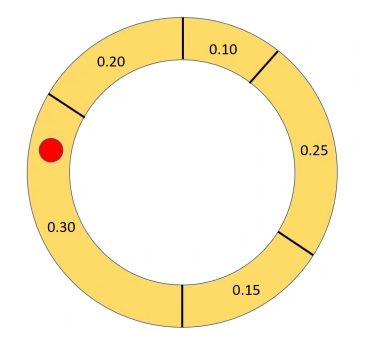
\includegraphics[width=9cm]{images/rulet.png}
\caption{Proporcionalna selekcija roditelja.}
\label{fig:rulet}
\end{figure}

Veliki brojevi predstavljaju problem, kod populacije s 5 rasporeda od kojih nakon transformacije svi imaju redom vrijednosti 10001, 10002, 10003, 10004 i 10005 razlike vjerojatnosti svakog rasporeda bit će zanemarive i svi rasporedi će efektivno imati vjerojatnost od 20\%. Kako bi se taj efekt ublažio, moguće je sve kazne iz populacije umanjiti vrijednošću za jedan manjom od najmanje vrijednosti. Tako sada redom vrijednosti iznose 1, 2, 3, 4, 5.

Sljedeći problem predstavljaju negativne vrijednosti, zbog nagrada koje rasporedi mogu poprimiti, kazna rasporeda može teoretski poprimiti negativnu vrijednost, zato je potrebno pronaći minimalnu vrijednost i u slučaju da je ta vrijednost negativna, svaki element se uveća za apsolutu vrijednost najmanje kazne.

Nadalje, vrijednosti svih kazni rasporeda u svakom krugu iteracije su skoro podjednake, stoga ako se u nizu nalazi velik broj rasporeda, svaki raspored imat će otprilike podjednaku šansu da bude odabran i tako se efektivno dobije nasumični odabir.

Nadalje, boljim rasporedom smatra se onaj koji ima manje kolizija, zbog toga je teško dodijeliti ispravnu vjerojatnost odabira, jedan način je da se umjesto kazne gleda broj kolizija, ali kada bi se broj kolizija smanjio na 0, svi rasporedi bi imali podjednaku vjerojatnost odabira.

Kada bi se sve ove adaptacije uvele u algoritam, jako bi usporio zbog velikog broja transformacija i kalkulacija prije samog odabira.

\subsection{Turnirska selekcija}

Turnirska selekcija kao ulaz u algoritam prima parametar \emph{k} koji označava broj jedinki koji ulaze u turnir. Vrlo jednostavnim postupkom, iz populacije se nasumično odabere \emph{k} rasporeda nakon čega se jednostavno vrati onaj koji ima najmanji broj preklapanja ili, u slučaju jednakog broja preklapanja, onaj s najmanjom kaznom.

\begin{algorithm}
\caption{Proporcionalna selekcija}
\label{algo:proporcionalno}
\begin{algorithmic}
\STATE{populacija := new raspored[k]}
\WHILE{size(populacija) != k}
\STATE{jedinka := odaberiNasumicno(rasporedi)}
\IF{populacija ne sadrži jedinku}
\STATE{dodaj(populacija, jedinka)}
\ENDIF
\ENDWHILE
\STATE{roditelj := odaberiNajbolji(populacija)}
\end{algorithmic}
\end{algorithm}

Kod punjenja pomoćne populacije, potrebno je provjeravati da se novo odabrani raspored već ne nalazi u populaciji.

\begin{figure}[htb]
\centering
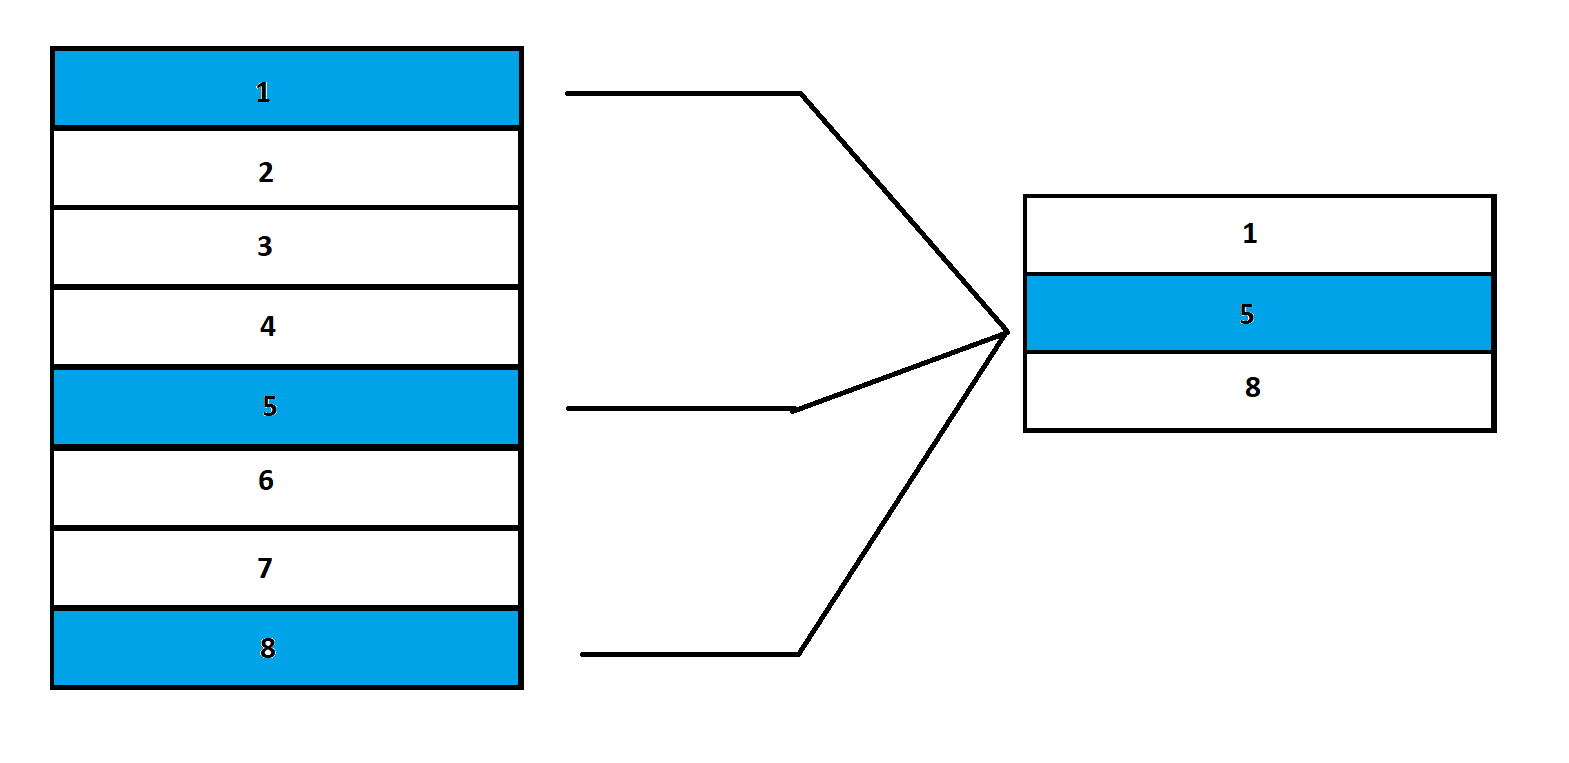
\includegraphics[width=14cm]{images/turnir.png}
\caption{Turnirska selekcija roditelja.}
\label{fig:turnir}
\end{figure}

Ako se za vrijednost \emph{k} u algoritmu postavi 1, onda je to efektivno odabir nasumičnog roditelja, a ako se za \emph{k} postavi veličina populacije, onda se odabire elitna jedinka. Za broj odabranih rasporeda postavlja se manja vrijednost poput 2 ili 3 kako bi se omogućilo barem minimalno svojstvo kompetencije.

Turnirska selekcija rješava problem velikih brojeva jer odabir rasporeda ne ovisi o razlici kazni pojedinih rasporeda. Dodatno, negativne vrijednost isto ne utječu na ispravnost algoritma kao niti veliki broj rasporeda u populaciji.

Zbog svoje jednostavnosti, efikasnosti i robusnosti, turnirska selekcija s parametrom tri je odabrana kao algoritam za odabir roditelja.

\section{Križanje roditelja}

Operator križanja roditelja, kao i operator odabira roditelja, sužava prostor pretrage. Križanjem dvaju roditelja nastaje jedno ili dva nova rješenja  ovisno o konkretnim implementacijama. Odabrano je da operator križanja kao rezultat vraća jedno dijete.

Različite implementacije daleko najmanje utječu na kvalitetu dobivenih rasporeda čak i kod ekstremnih postavka operatora.

\subsection{Nasumično križanje}

Nasumičnim križanjem, za svaki element iz rasporeda postoji 50\% šanse da bude odabran bilo koji od oba roditelja za dohvat tog elementa.

\begin{figure}[htb]
\centering
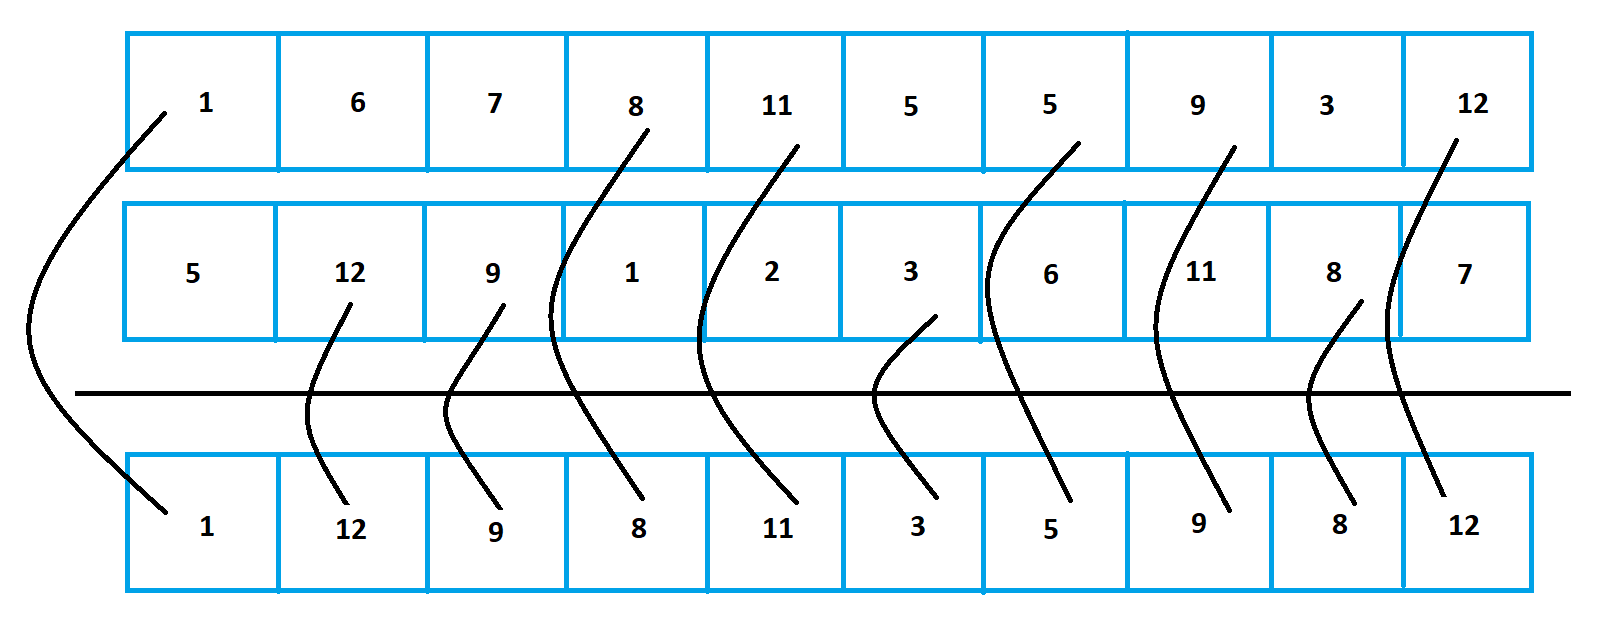
\includegraphics[width=14cm]{images/rand_cross.png}
\caption{Nasumično križanje.}
\label{fig:rand_cross}
\end{figure}

\subsection{Alternirajuće križanje}

Različito od nasumičnog križanja, ovdje je slučajnost pristupna samo jednom, za odabir roditelja od kojeg počinje križanje. Nadalje, ovisno o parametru \emph{k} koji je predan algoritmu, djetetu se postavlja idućih \emph{k} vrijednosti odabranog roditelja te se potom roditelj mijenja i od njega se uzima idućih \emph{k} vrijednosti i tako sve dok se ne popune svi elementi dijeteta.

\begin{figure}[htb]
\centering
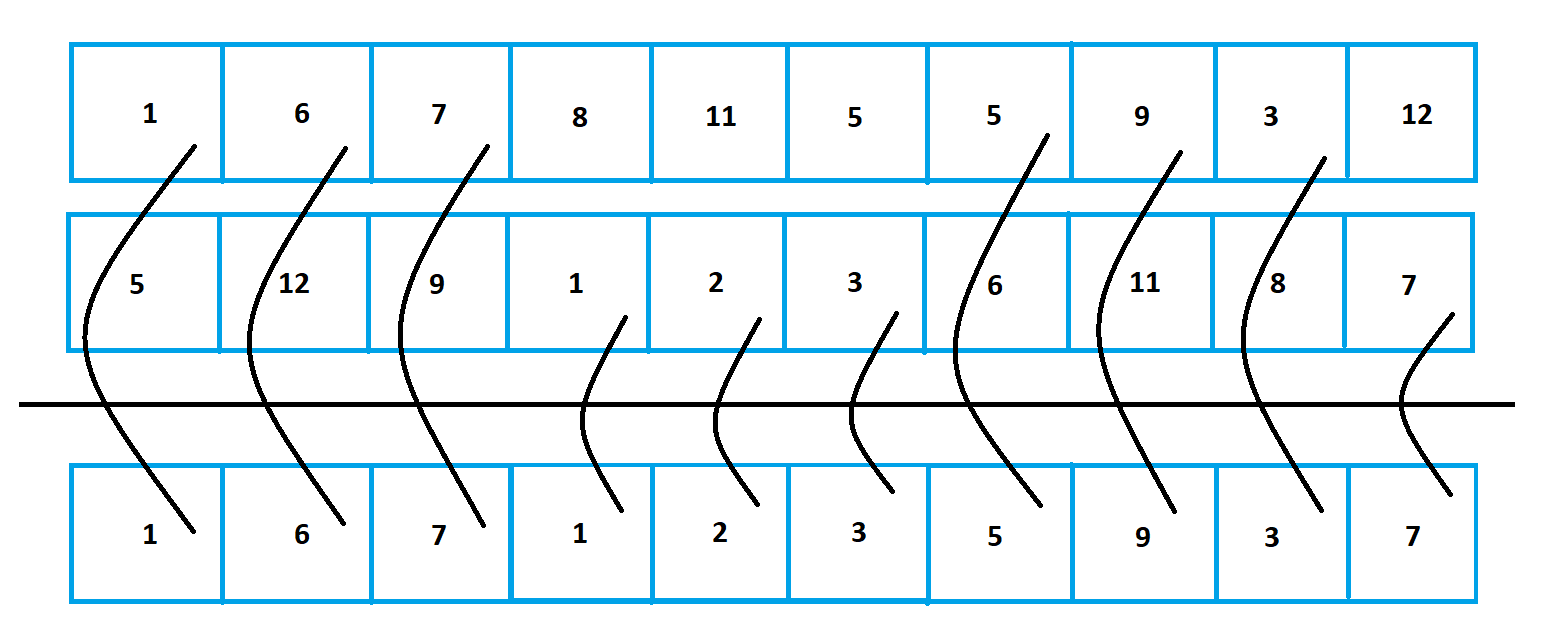
\includegraphics[width=14cm]{images/cross_alt.png}
\caption{Alternirajuće križanje s K = 3.}
\label{fig:cross_alt}
\end{figure}

Ako se kao parametar \emph{k} postavi jedinica, onda se redom uzima termin jednog, pa termin drugog roditelja naizmjence.

\begin{figure}[htb]
\centering
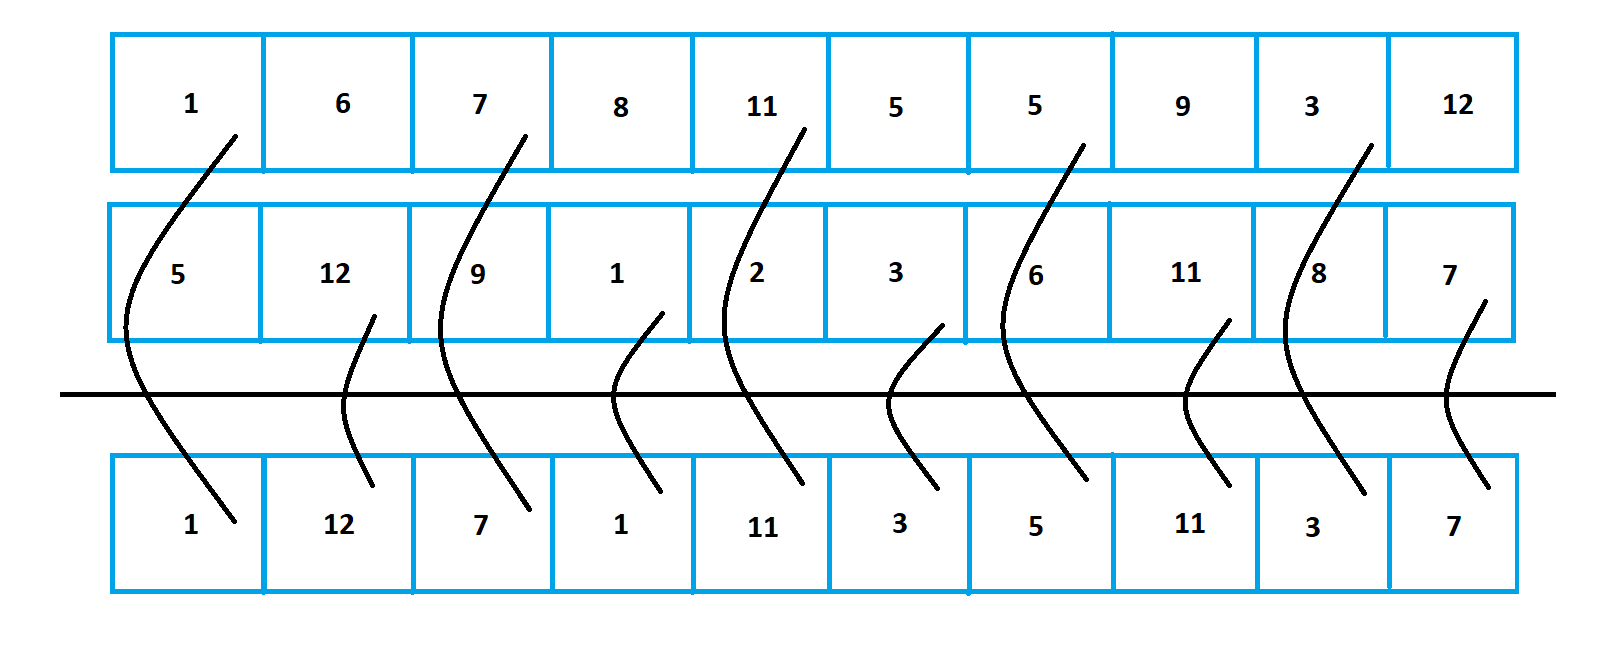
\includegraphics[width=14cm]{images/cross_alt_1.png}
\caption{Alternirajuće križanje s K = 1.}
\label{fig:cross_alt_1}
\end{figure}

Sljedeći posebni slučaj je ako se za parametar \emph{k} postavi vrijednost N/2, onda algoritam jednostavno uzme polovicu svakog roditelja. Također, ispravno je nazvati ovaj slučaj križanje s polovičnom točkom prekida.

\begin{figure}[htb]
\centering
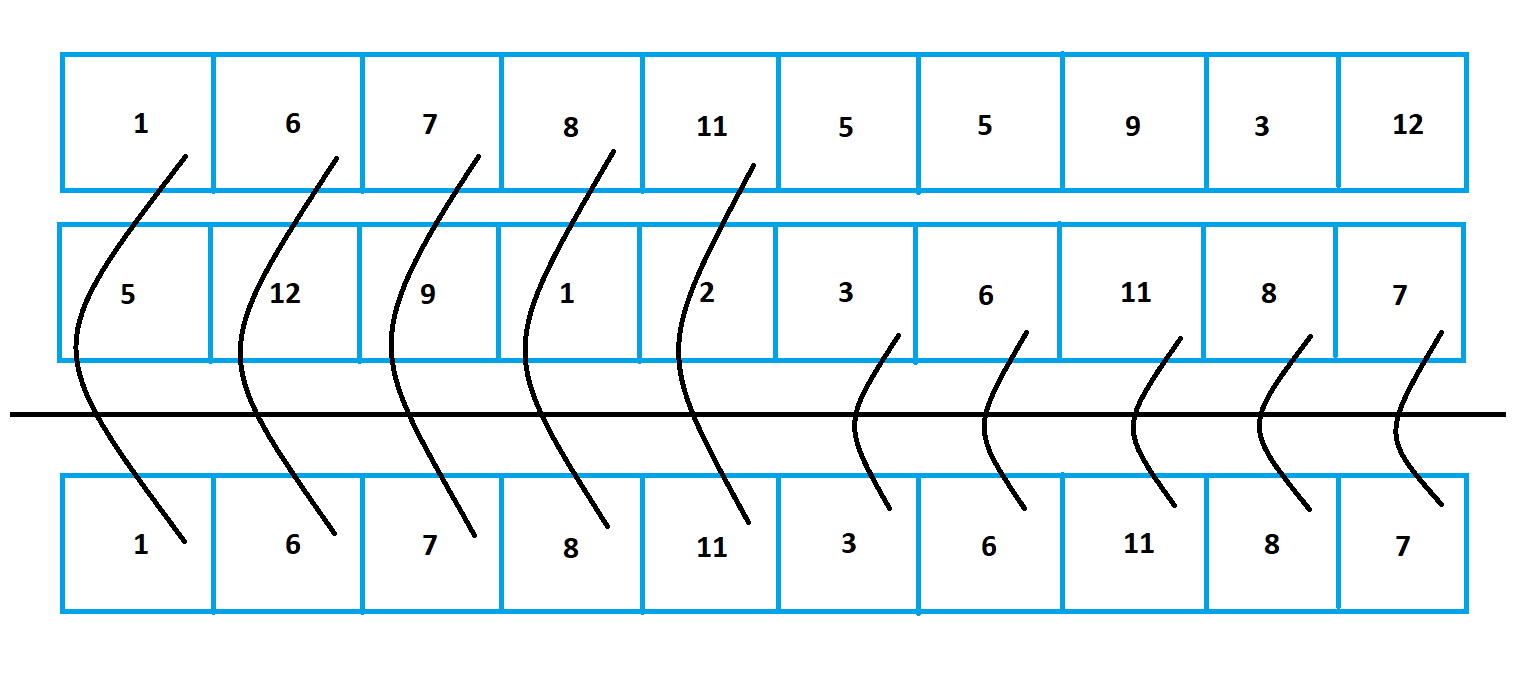
\includegraphics[width=14cm]{images/half_cross.png}
\caption{Alternirajuće križanje s K = N/2.}
\label{fig:half_cross}
\end{figure}

\newpage

Posljednje, ako se za parametar \emph{k} odabere vrijednost veća od N/2, onda ovo postaje križanje s točkom prekida. Jedina razlika na sami algoritam križanja točkom prekida je što nisu dostupne točke prekida manje od N/2.

\section{Mutacija}

Osim operatora koji sužavaju područje pretrage, mutacija ga proširuje. Bez operatora mutacije, vrlo brzo bi sva nova rješenja počela stagnirati, tj. ne bismo dobili više novih rješenja. Operatoru je dodijeljena stopa mutacije, postotak studenata za koji će se promijeniti dodijeljeni termin.

Optimalna vrijednost mutacije  iznosi oko 0.002 ili 0.2\%. Raspored se sastoji od termina za 831 studenta, prema tome, nakon svake mutacije će se u prosjeku promijeniti grupa za 1.66 studenata što pruža dovoljno jako svojstvo širenja. Uz veće vrijednosti stope mutacije, konvergencija je sporija bez poboljšanja u kvaliteti rješenja.

Kod ovog problema nije potrebno pronaći najbolje moguće rješenje, već dovoljno dobro. Zato i s jako malim stopama promjene, kad algoritam ima veću vjerojatnost zapeti u lokalnom, rješenje se smatra prihvatljivim.

\subsection{Promjena termina za fiksan broj mjesta}

Jedna od varijanti mutacije je promjena termina za fiksan broj mjesta. Na primjer, studenta se prebaci s termina 8 na termin 11.

\begin{figure}[htb]
\centering
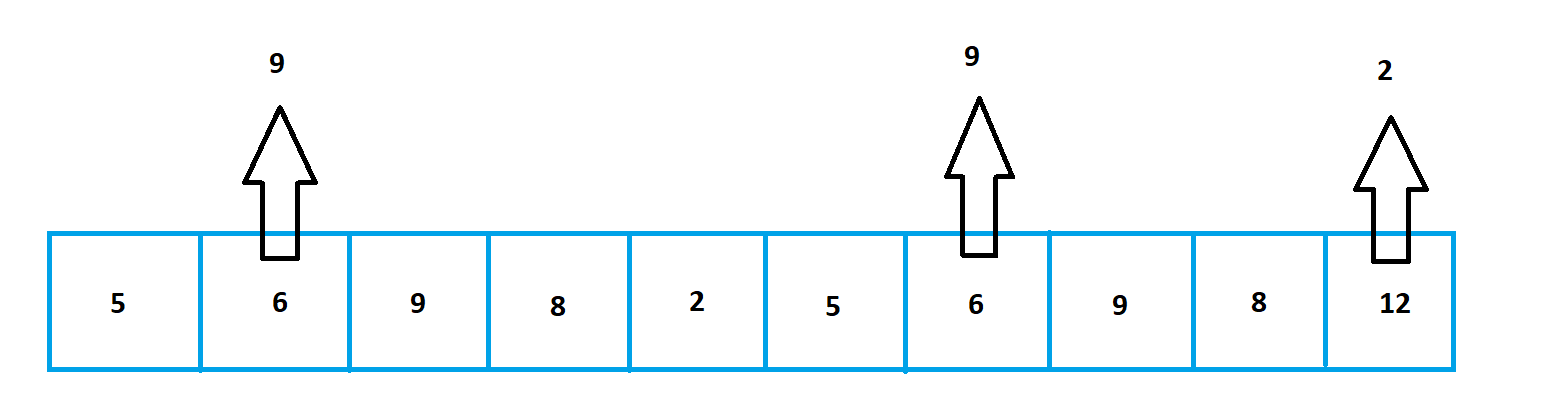
\includegraphics[width=15cm]{images/mut_3.png}
\caption{Mutacija uvećanjem termina za fiskan broj K = 3.}
\label{fig:mut_3}
\end{figure}

Ovako definiran operator kasnije u ciklusu pretrage, kad se raspored stabilizira i većina termina imaju popunjen kapacitet od 15 ili 16 mjesta, radi velik broj promjena što destabilizira ponašanje. Ako se napravi promjena termina za 2 studenta, pogotovo ako su oni u istoj grupi, novi raspored će vrlo vjerojatno imati veću kaznu. Prilikom promjene termina primjenjuje se formula:

\begin{equation}
\forall i\ termin[i] = (termin[i] + N)\mod brojTermina
\label{eq:trans-kazne}
\end{equation}

Kao što se vidi na slici \ref{fig:mut_3}, 2.\ i 7.\ termin se povećavaju sa 6 na 9 i 10.\ sa 12 na 2 zbog utjecaja operatora \emph{mod}.

\subsection{Nasumičan odabir termina}

Nasumičan odabir termin radi tako da se studentu dodijeli nasumično generiran broj termina između 0 i \emph{brojTermina} gdje svaki termin ima jednaku šansu biti odabran.

\begin{figure}[htb]
\centering
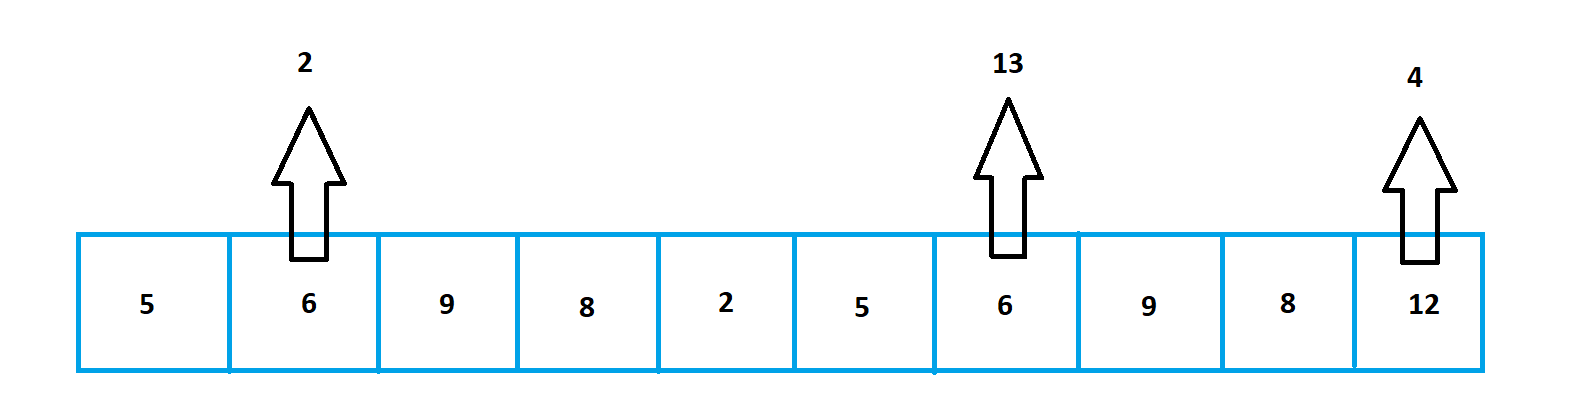
\includegraphics[width=15cm]{images/mut_rand.png}
\caption{Mutacija dodjelom nasumičnog termina.}
\label{fig:mut_rand}
\end{figure}

Dodjelom nasumičnog termina umjesto pomaka termina za fiksni broj mjesta bolje rješava problem potencijalnog nakupljanja termina na jednom mjestu pa je odabran kao operator mutacije.

\section{Veličina populacije}

Veličina populacije je broj rasporeda koji se u svakom trenu čuva u memoriji. S manjom veličinom populacije povećava se broj iteracija po sekundi, ali je zato manja raznolikost rješenja. No s većom veličinom populacije smanjit će se broj iteracija po sekundi, ali će se povećati raznolikost rješenja te će se potencijalno pronaći bolje rješenje.

Operacije računanja kazne su skupe zbog velikog broja provjera kroz koje je potrebno proći pa će se s većom populacijom broj iteracija po sekundi drastično smanjiti. Potrebno je pronaći dobar balans kvalitete i brzine. Kroz testiranje, vrijednosti oko 25 su se pokazale jako dobre.

\chapter{Usporedba rezultata}

U ovom poglavlju bit će potkrijepljeni razni parametri odabrani kroz ostatak rada, razlike između različitih algoritama, rad konfigurabilnih algoritama ovisno o parametrima i brzina izvođenja ovisno o parametrima. Prilikom testiranja uzimaju se sljedeće pretpostavke, osim ako je navedeno drugačije:

\begin{itemize}
	\item iznosi kazne:
	\begin{itemize}
		\item previše studenata u terminu je kvadriran broj studenata pomnožen s 95
		\item premalo studenata u terminu  je kvadriran broj studenata pomnožen s 45
		\item preklapanje iznosi 150
		\item slijedni termin iznosi -5
		\item pauza između termina nastala zbog odabranog termina je 2 pomnoženo s kvadriranim brojem sati
		\item termin dodijeljen u danu bez ostalih nastavnih obveza iznosi 100
	\end{itemize}	
	\item algoritam je elitistički
	\item odabir roditelja je turnir s parametrom 3
	\item dijete nastaje nasumičnim križanjem roditelja
	\item mutacija nasumično odabire termin sa stopom mutacije 0.002
	\item bolji je onaj raspored koji ima manje preklapanja i onaj koji ima manju kaznu
	\item algoritam staje nakon 3000 iteracija
	\item 831 student se dijeli u 43 termina.
\end{itemize}

\section{Vrijednosti odabrane za izračun kazne}

Smanjivanjem kazne, algoritam je u ranijim iteracijama više sklon praznijim grupama ili grupama od nekoliko studenata. Provodi se ispitivanje o broju termina s prekršenim ograničenjem minimalnog kapaciteta i maksimalnog kapaciteta. Ispitivanje se radi na 1000 iteracija.

\begin{table}[htb]
\caption{Popunjenost termina ovisno o kazni nezadovoljavanja minimlanog kapaciteta.}
\label{tbl:min-popunjenost}
\centering
\begin{tabular}{lll} \hline
kazna & 14 ili manje &  17 ili više \\ \hline
15 & 3 & 22 \\
30 & 4 & 19 \\
45 & 3 & 18 \\
55 & 5 & 16 \\ \hline
\end{tabular}
\end{table}

Iz tablice je vidljivo kako kazne s vrijednošću 45 i 55 imaju najbolja svojstva, kazna od 55 je odabrana kako svejedno pri većem broju iteracija ne bi toliko bili preferirani termini s manjim brojem studenata.

Isti postupak se provodi za kaznu s prekršenim maksimalnim kapacitetom s 1500 iteracija.

\begin{table}[htb]
\caption{Popunjenost termina ovisno o kazni nezadovoljavanja maksimalnog kapaciteta.}
\label{tbl:max-popunjenost}
\centering
\begin{tabular}{lll} \hline
kazna & 14 ili manje &  17 ili više \\ \hline
50 & 6  & 11  \\
75 & 5 & 12 \\
95 & 2 & 6 \\
110 & 2 & 13 \\ \hline
\end{tabular}
\end{table}

Vrijednost kazne od 95 konzistentno pokazuje najbolja svojstva te je upravo iz tog razloga odabrana.

Nadalje slijedi ispitivanje o brzini minimizacije preklapanja ovisno o kazni.  Prilikom ispitivanja broj iteracija je postavljen na 100.

Iz grafova je moguće primijetiti kako kazna preklapanja nema velik utjecaj na algoritam, zbog turnirske selekcije dominira odabir rasporeda s manjim brojem preklapanja.

\begin{figure}
    \centering
    \subfigure[]{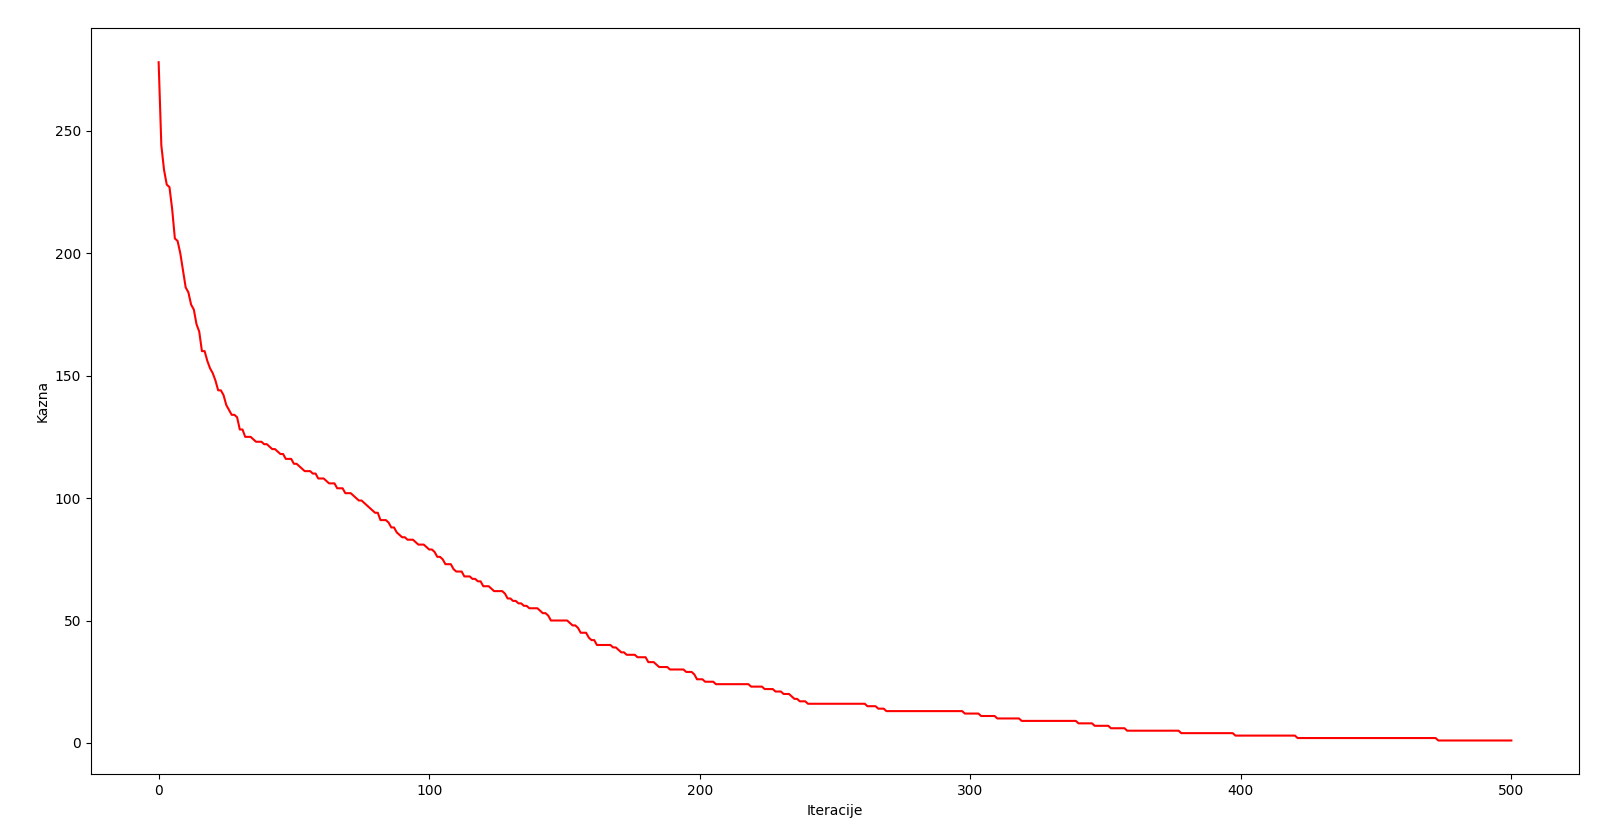
\includegraphics[width=0.45\textwidth]{images/preklapanje_25.png}} 
    \subfigure[]{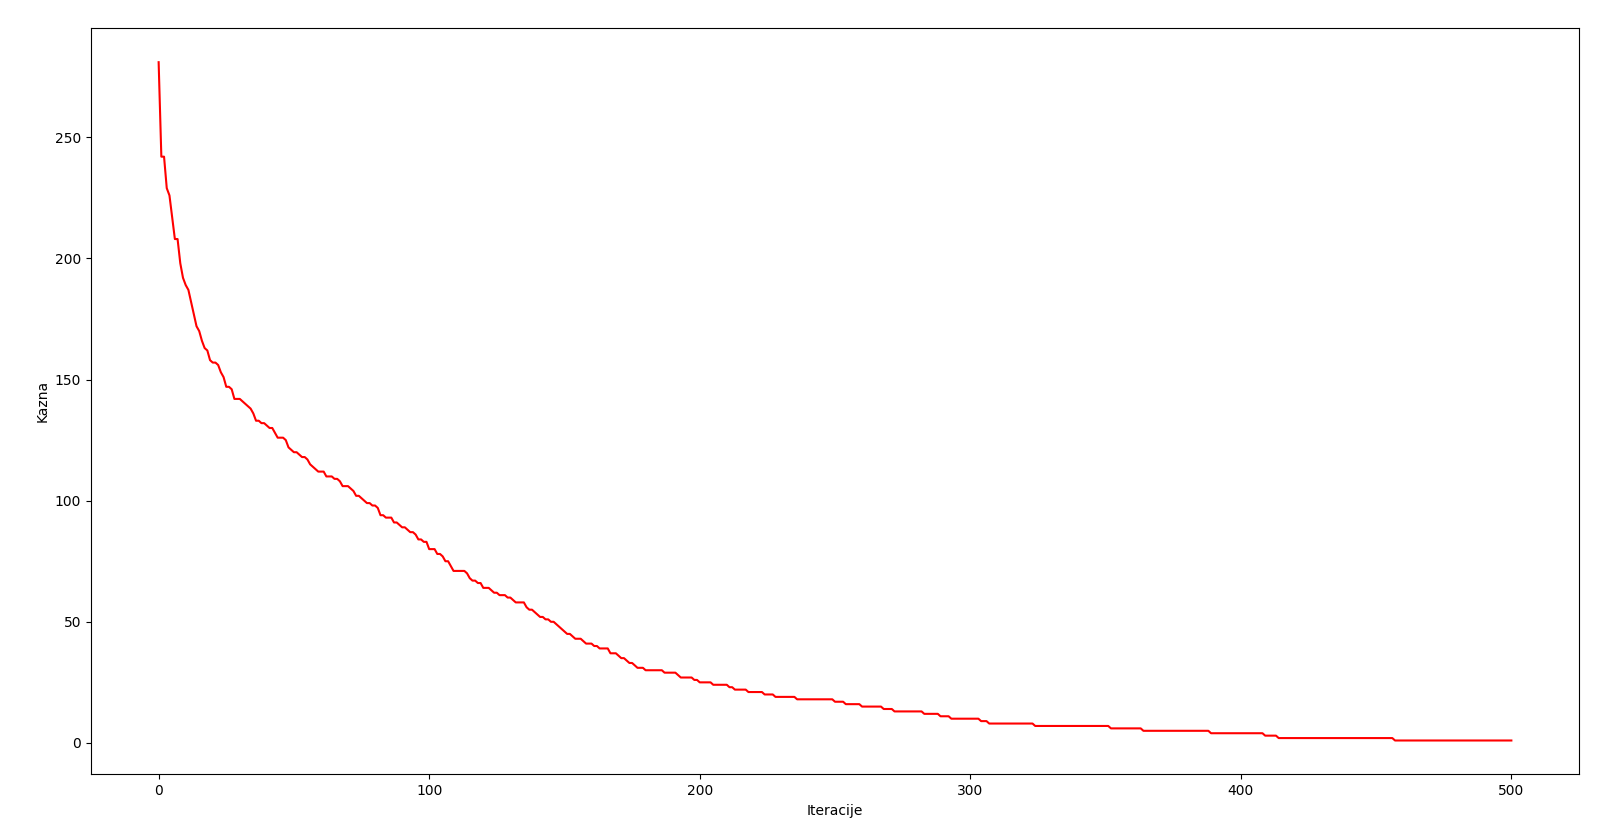
\includegraphics[width=0.45\textwidth]{images/preklapanje_150.png}} 
    \subfigure[]{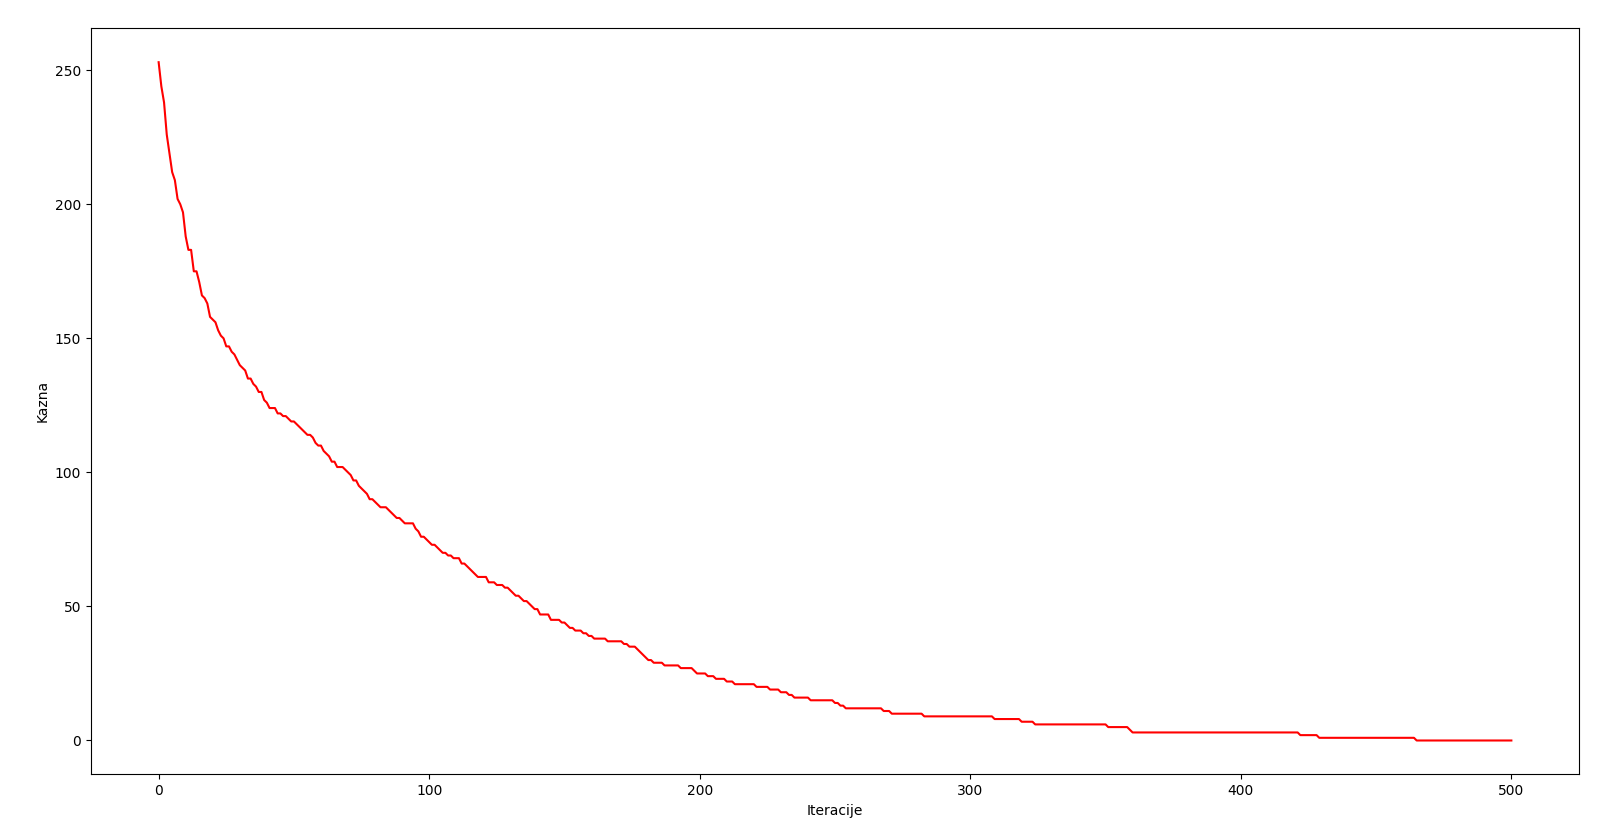
\includegraphics[width=0.45\textwidth]{images/preklapanje_250.png}}
    \caption{(a) kazna = 25 (b) kazna = 150 (c) kazna = 250}
    \label{fig:kazne}
\end{figure}
\newpage

Također, ispituje se i nagrada, teško je ispitati razliku u kazni rasporeda jer će rasporedi s većom nagradom prirodno imati manju kaznu i obrnuto, ali raspored manje kazne u tom slučaju ne mora biti bolje kvalitete. Stoga se ispituje broj prekršenih ograničenja kapaciteta termina laboratorijskih vježbi kako bi se pokazalo da su rasporedi s manjom nagradom skloniji boljim rješenjima.

\begin{table}[htb]
\caption{Prekršena ograničenja kapaciteta ovisno o nagradi slijednih temina.}
\label{tbl:nagrada}
\centering
\begin{tabular}{ll} \hline
nagrada &  prekršena ograničenja\\ \hline
1 & 4  \\
5 & 5 \\
15  & 7 \\
25 & 6 \\ \hline
\end{tabular}
\end{table}

U tablici se nalaze prosječne vrijednosti termina s prekršenim ograničenjima, nagrada iznosa 5 je odabrana jer pruža mali broj termina s prekršenim ograničenjima, a rasporedima ipak dodjeljuje dobra svojstva.

\section{Elitizam i odabir roditelja}

Kod promatranja elitizma, razlike između elitističke i neelitističke varijante su relativno male, ipak s uključenim elitizmom rasporedi imaju manje varijacije i brže konvergiraju što je vidljivo na grafovima. Prvih 500 iteracija je odrezano na prikazima.

\begin{figure}[htb]
\centering
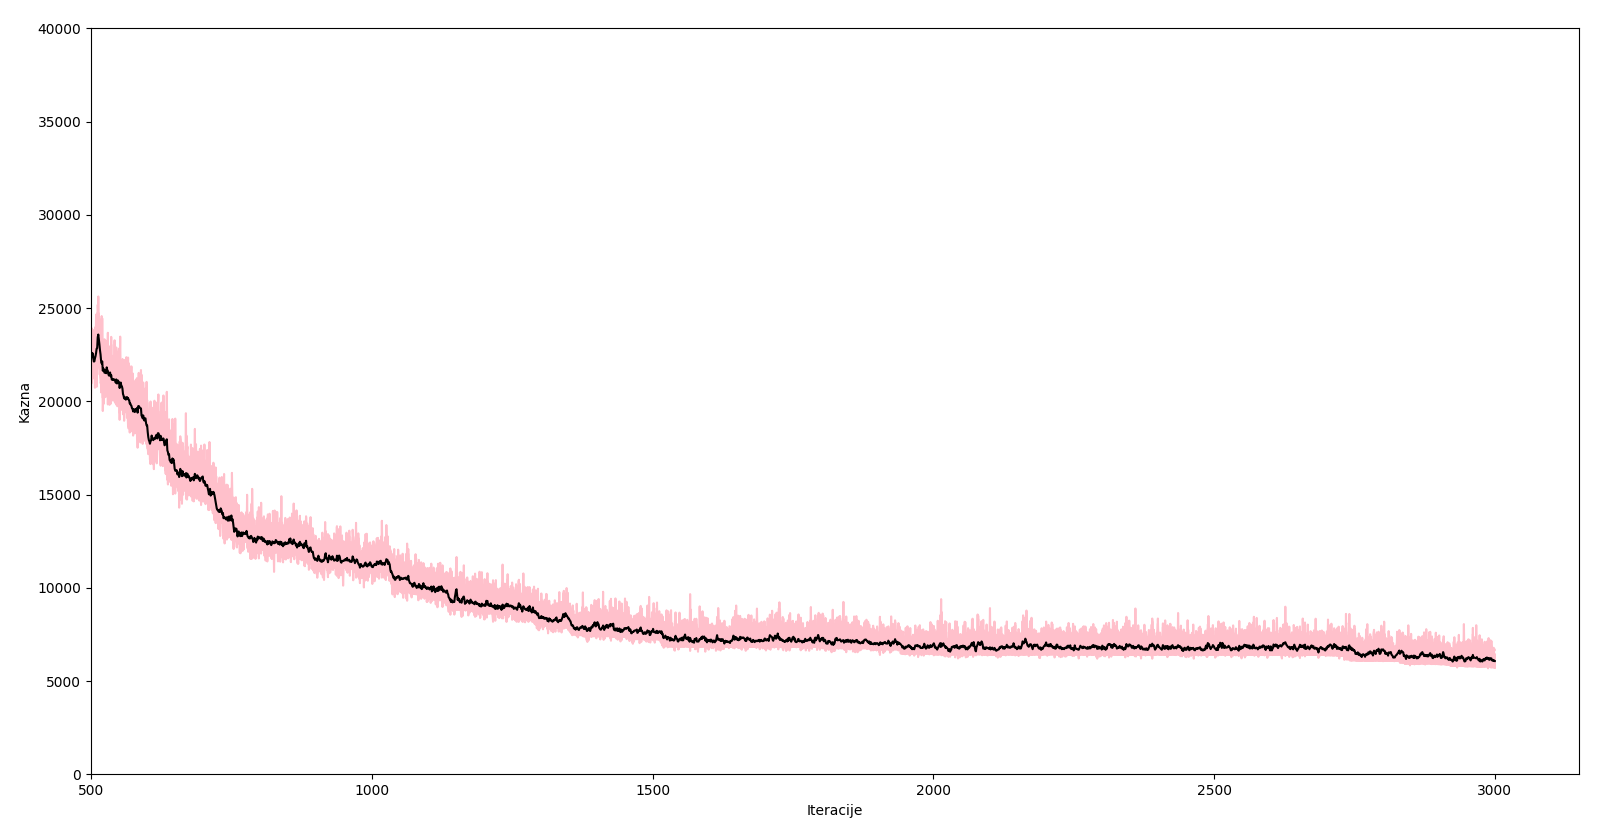
\includegraphics[width=14cm]{images/usp_elitizam_da.png}
\caption{Rasporedi s uključenim elitizmom.}
\label{fig:usp_elitizam_da}
\end{figure}

\begin{figure}[htb]
\centering
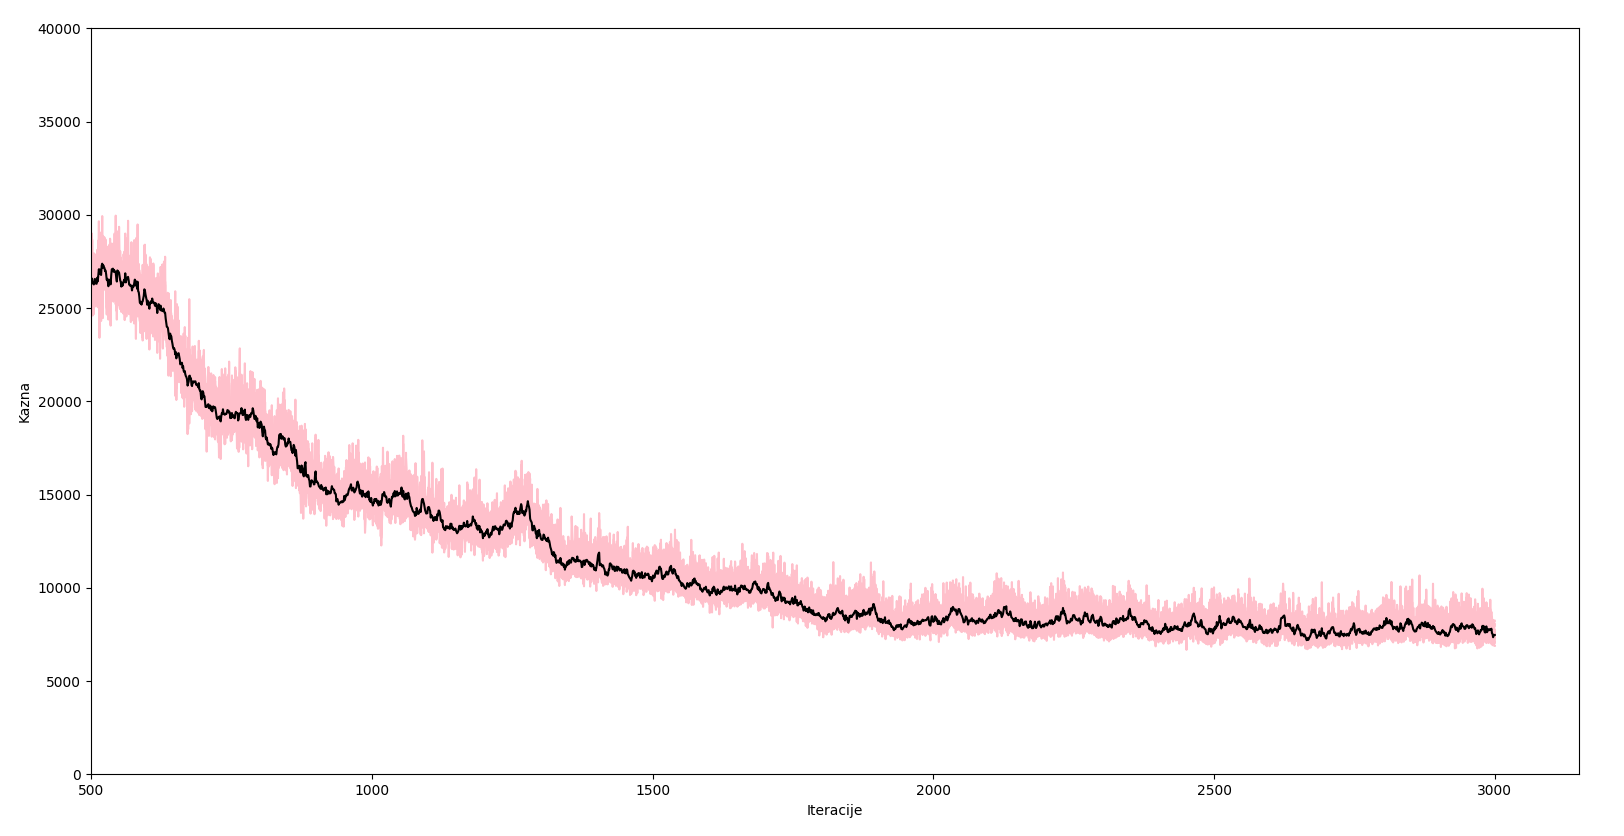
\includegraphics[width=14cm]{images/usp_elitizam_ne.png}
\caption{Rasporedi s isključenim elitizmom.}
\label{fig:usp_elitizam_ne}
\end{figure}

Elitistički algoritam u 3000 iteracija dostigne kaznu od oko 5500 dok neelitistička inačica završi na oko 7500.

Bez elitizma odabir roditelja s verzijom proporcionalnog odabira sa svim modifikacijama  kako bi odabir bio što bolji, populacijom veličine 10 što pospješuje dodatno uspjeh proporcionalne selekcije i 10000 iteracija i dalje ne pronalazi raspored bez preklapanja. Broj preklapanja varira oko 10 preklapanja te rasporedi zapinju u lokalnom optimumu s kaznom koja iznosi oko 20000.

Ako se umjesto unaprijeđene verzije proporcionalne selekcije koristi osnovna verzija, bez korekcije velikih i negativnih brojeva te također bez elitizma, rezultati su još gori, prosječan broj preklapanja nakon 10000 iteracija iznosi oko 250 i kazna poprima vrijednosti oko 60000.

\begin{figure}[htb]
\centering
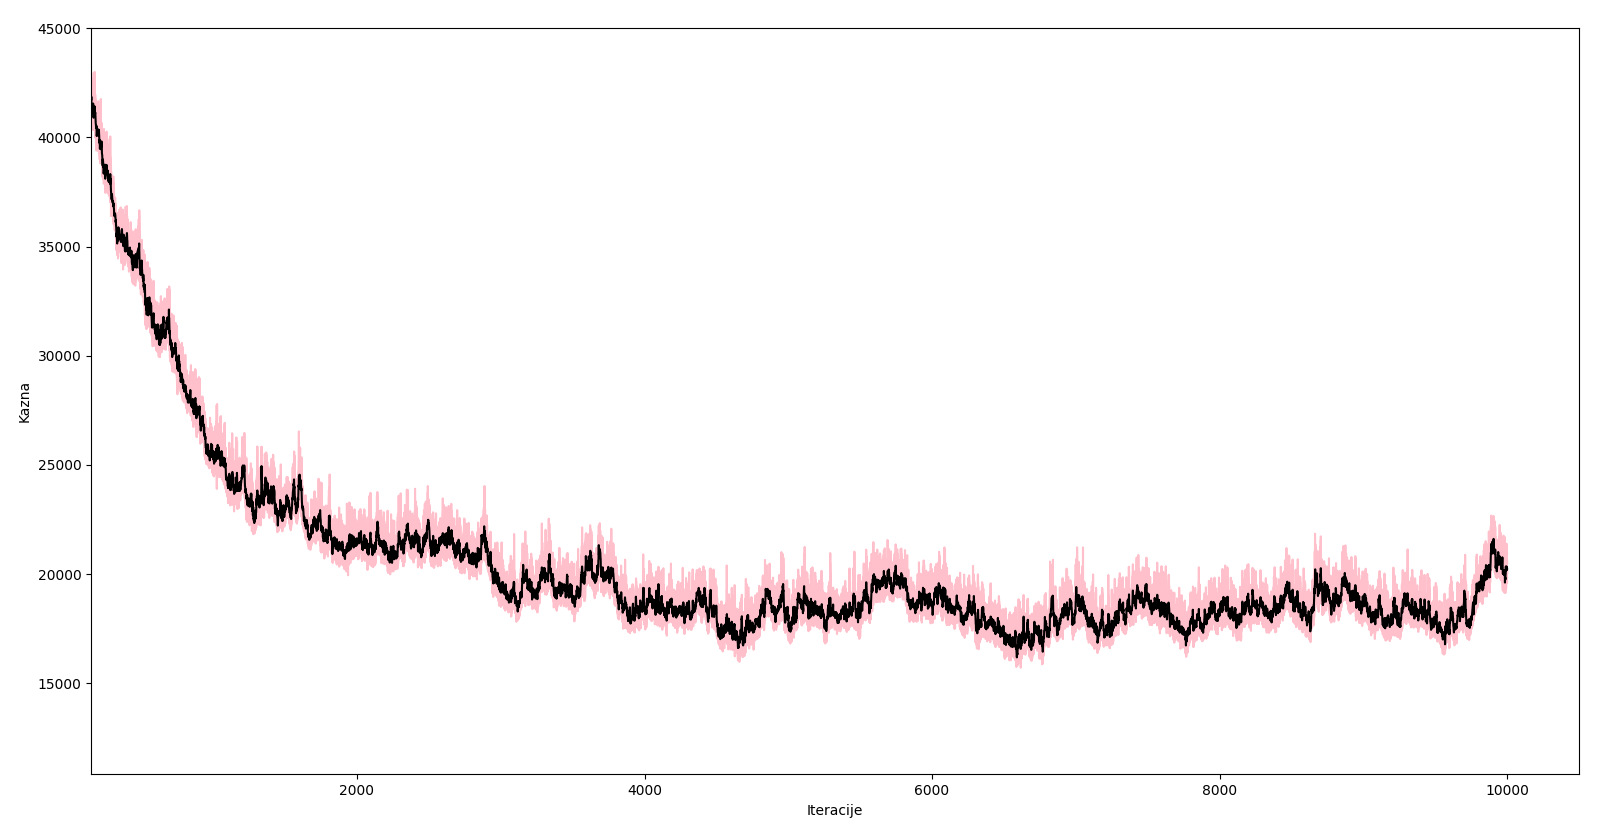
\includegraphics[width=14cm]{images/proporcije_e_ne.png}
\caption{Poboljšana verzija proprocionalne selekcije s isključenim elitizmom.}
\label{fig:prop_e_ne}
\end{figure}

\begin{figure}[htb]
\centering
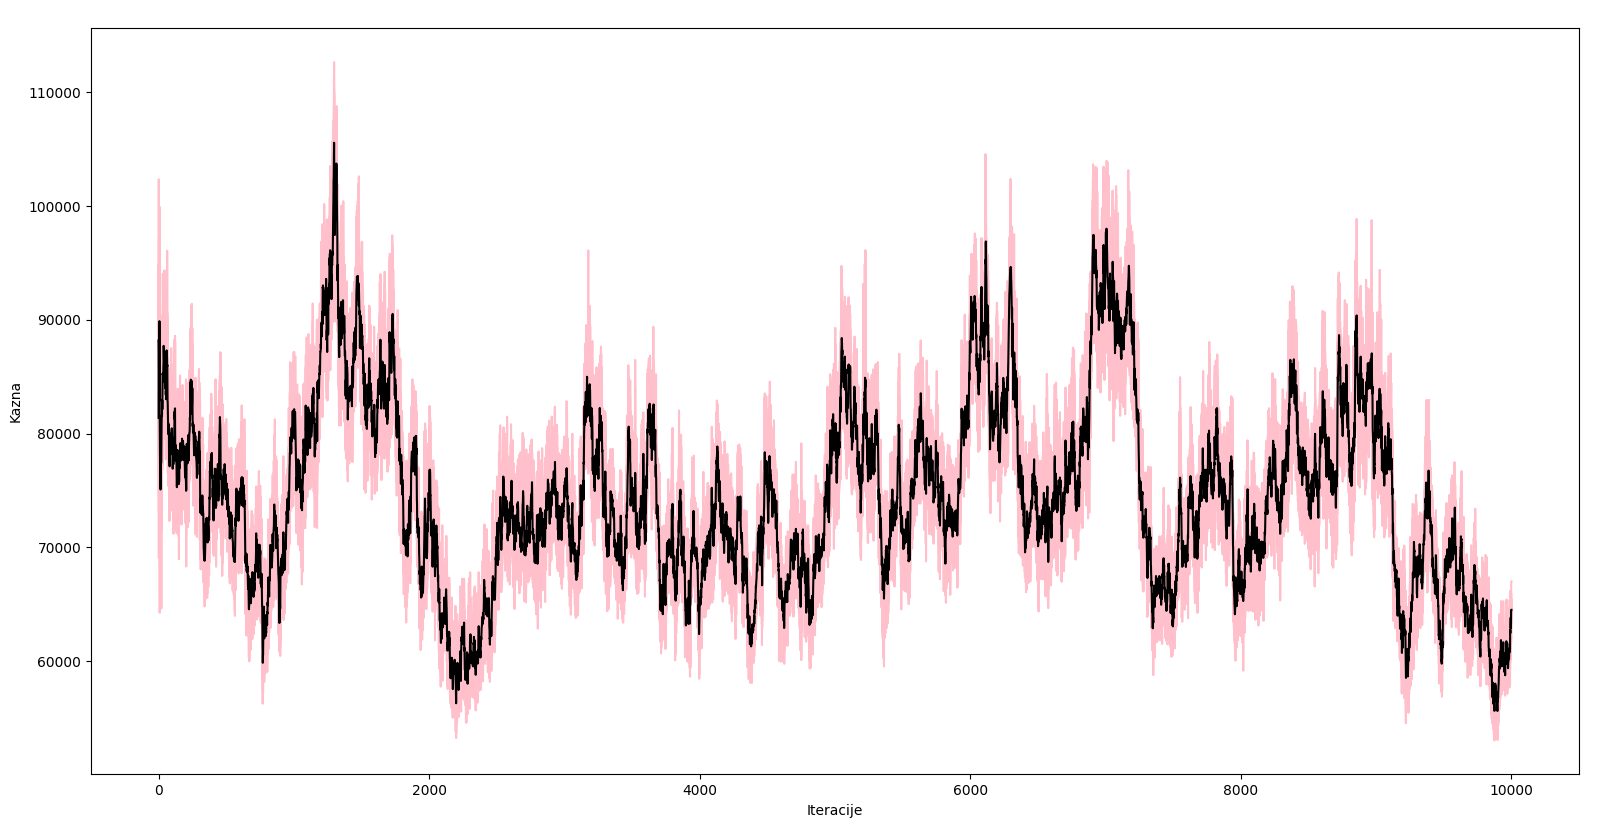
\includegraphics[width=14cm]{images/proporcije_e_ne_gore.png}
\caption{Osnovna verzija proprocionalne selekcije s isključenim elitizmom.}
\label{fig:proporcije_e_ne_gore}
\end{figure}

\newpage

Kod poboljšane verzije odabira proporcijom uključivanjem elitizma vrijednosti se smanjuju nakon 10000 iteracija s 20000 na vrijednosti oko 12000, dok broj kolizija ostaje relativno jednak. Osnovna verzija postiže drastično bolje vrijednosti, nakon 1500 iteracija se broj kolizija smanjuje na oko 50, ali tu algoritam zapne u lokalnom optimumu i dalje zastaje na kazni od oko 25000.

Usporedba rada turnirske selekcije s elitizmom i bez njega već je prethodno prikazana na slikama \ref{fig:elitiziam_da} i \ref{fig:elitiziam_ne}.

\begin{figure}[htb]
\centering
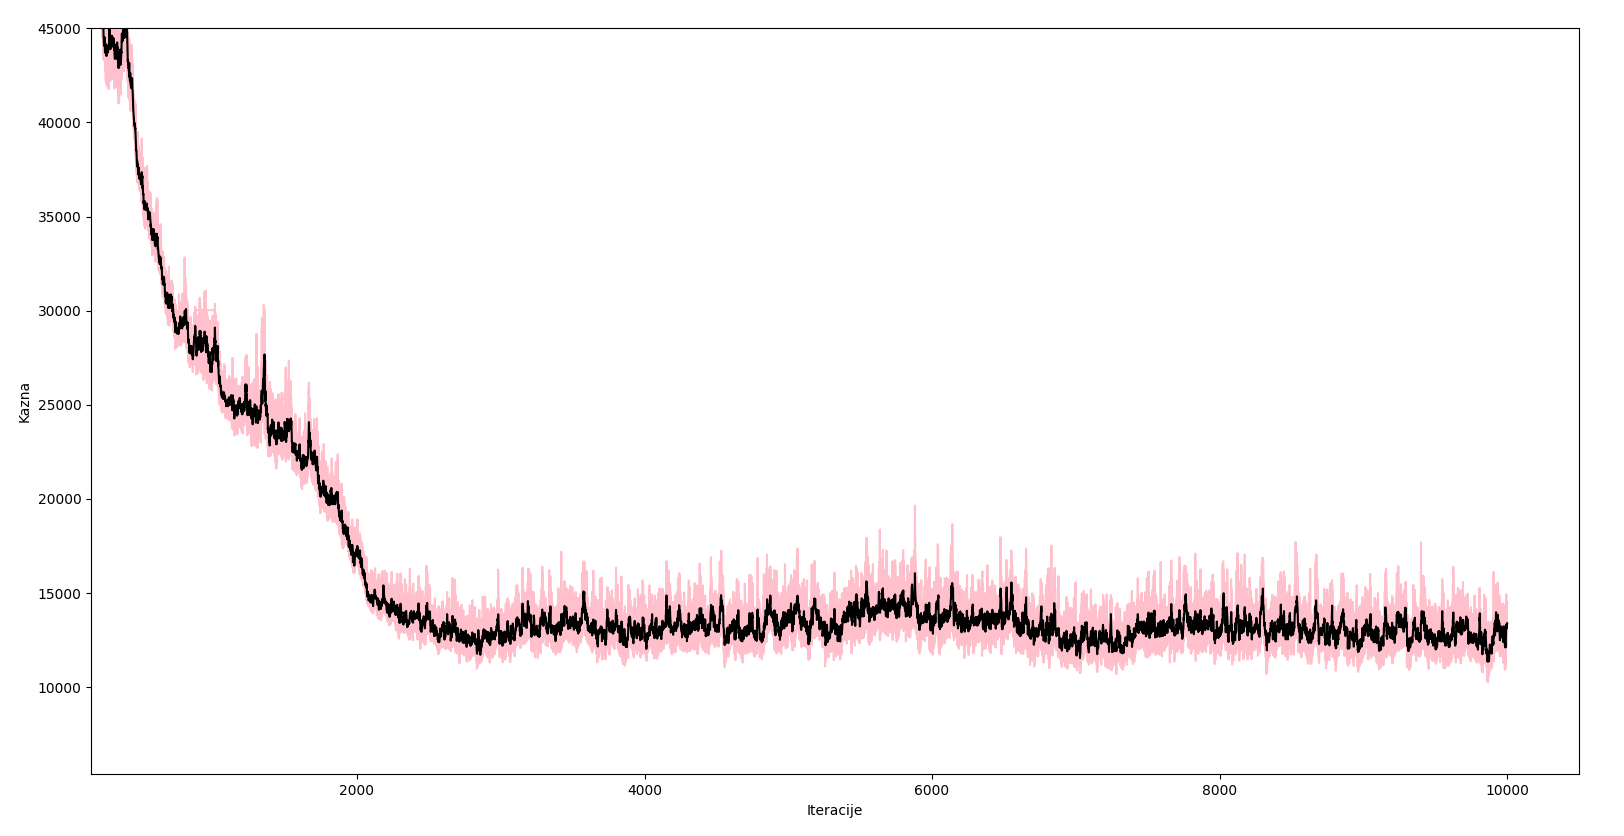
\includegraphics[width=14cm]{images/proporcije_e_da.png}
\caption{Poboljšana verzija proprocionalne selekcije s uključenim elitizmom.}
\label{fig:prop_e_da}
\end{figure}


\begin{figure}[htb]
\centering
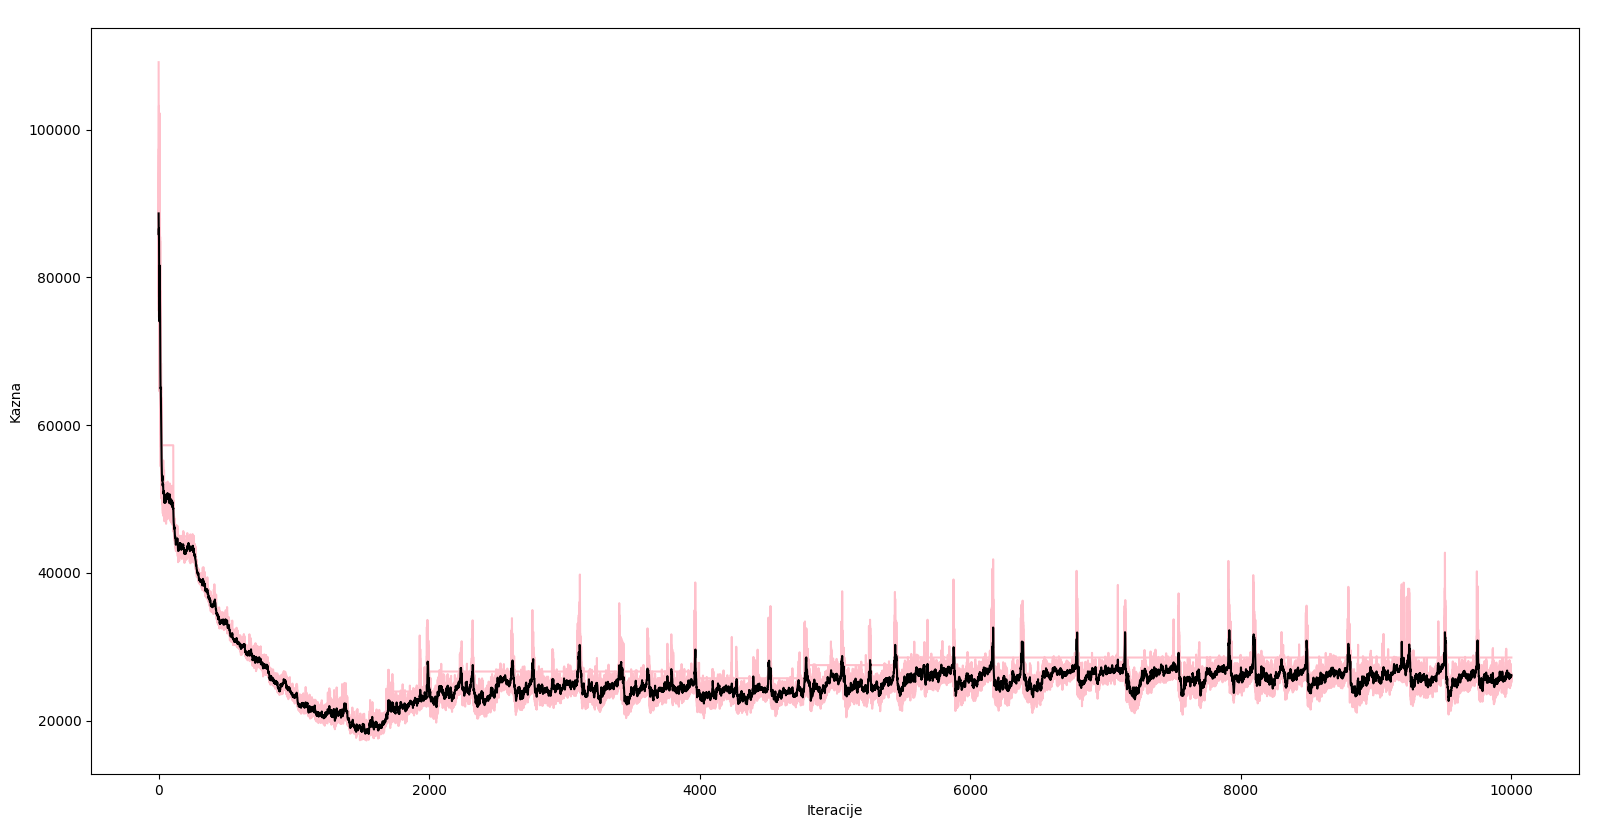
\includegraphics[width=14cm]{images/proporcije_e_da_gore.png}
\caption{Osnovna verzija proprocionalne selekcije s uključenim elitizmom.}
\label{fig:proporcije_e_da_gore}
\end{figure}

\section{Mutacija}

Rezultati mutacije odabirom nasmičnog termina vježbi vidljivi su na slici \ref{fig:elitiziam_da}, dok promjena termina za fiksnu vrijednost jednakoj 3 zapinje na oko 30 kolizija i na kazni oko 75000.

\begin{figure}[htb]
\centering
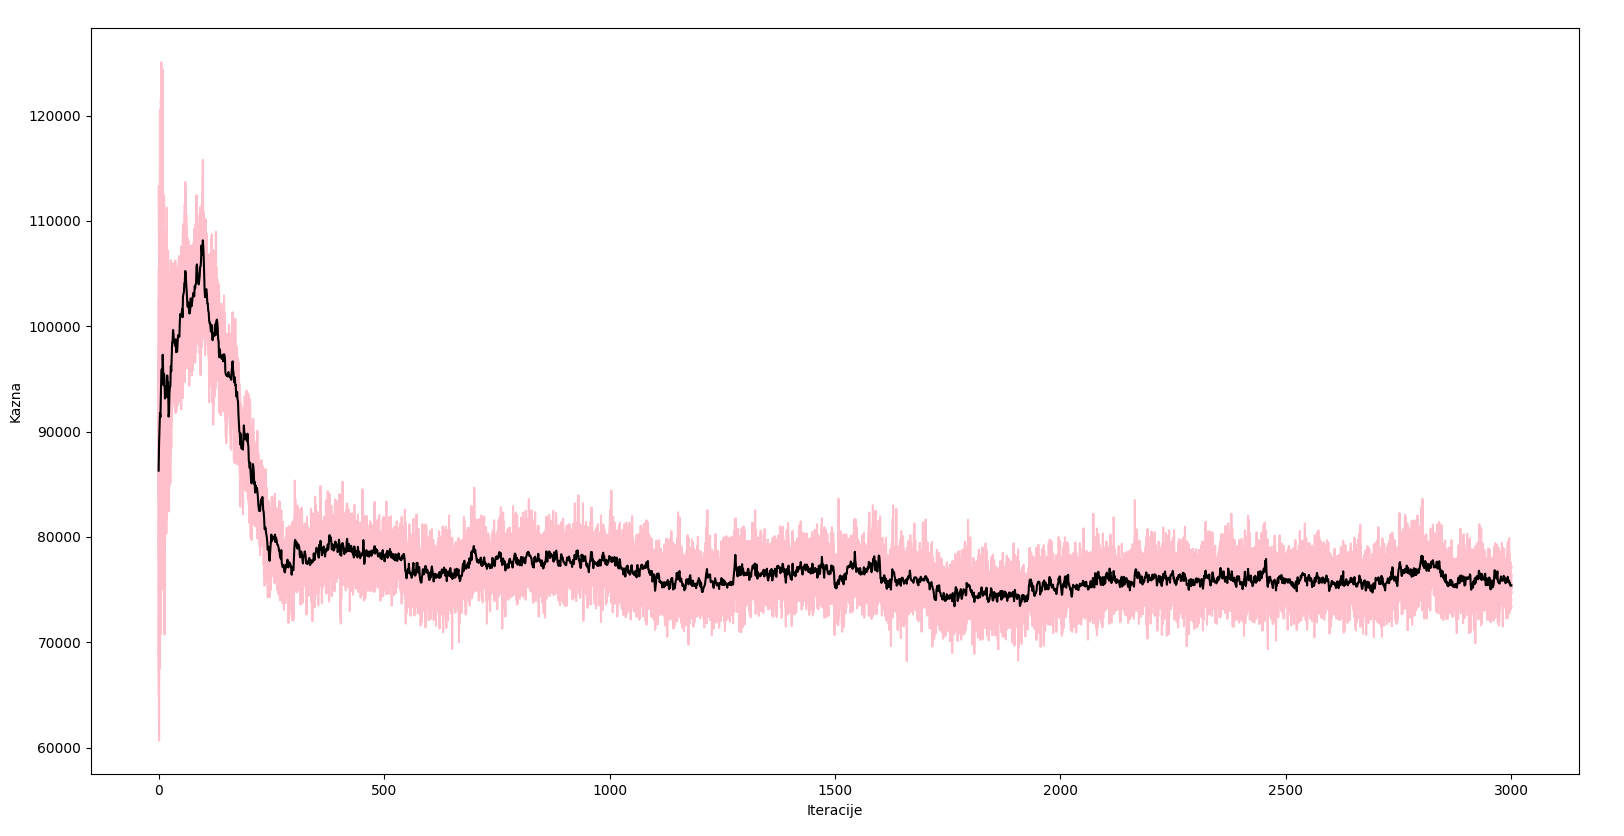
\includegraphics[width=15cm]{images/plus_tri.png}
\caption{Mutacija promjenom termina za fiksni broj mjesta.}
\label{fig:plus_tri}
\end{figure}

\section{Križanje}

\begin{figure}[htb]
    \centering
    \subfigure[]{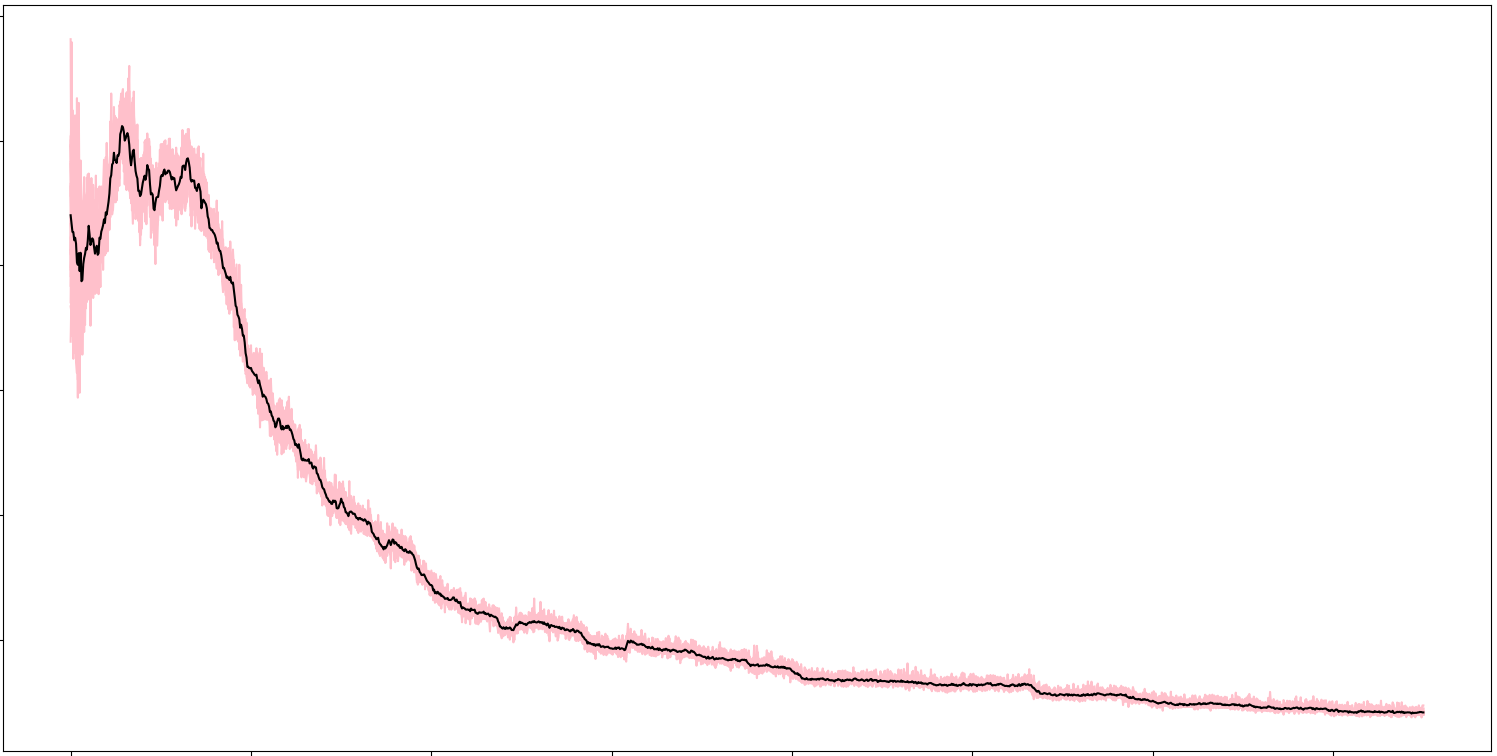
\includegraphics[width=0.35\textwidth]{images/cross_random.png}} 
    \subfigure[]{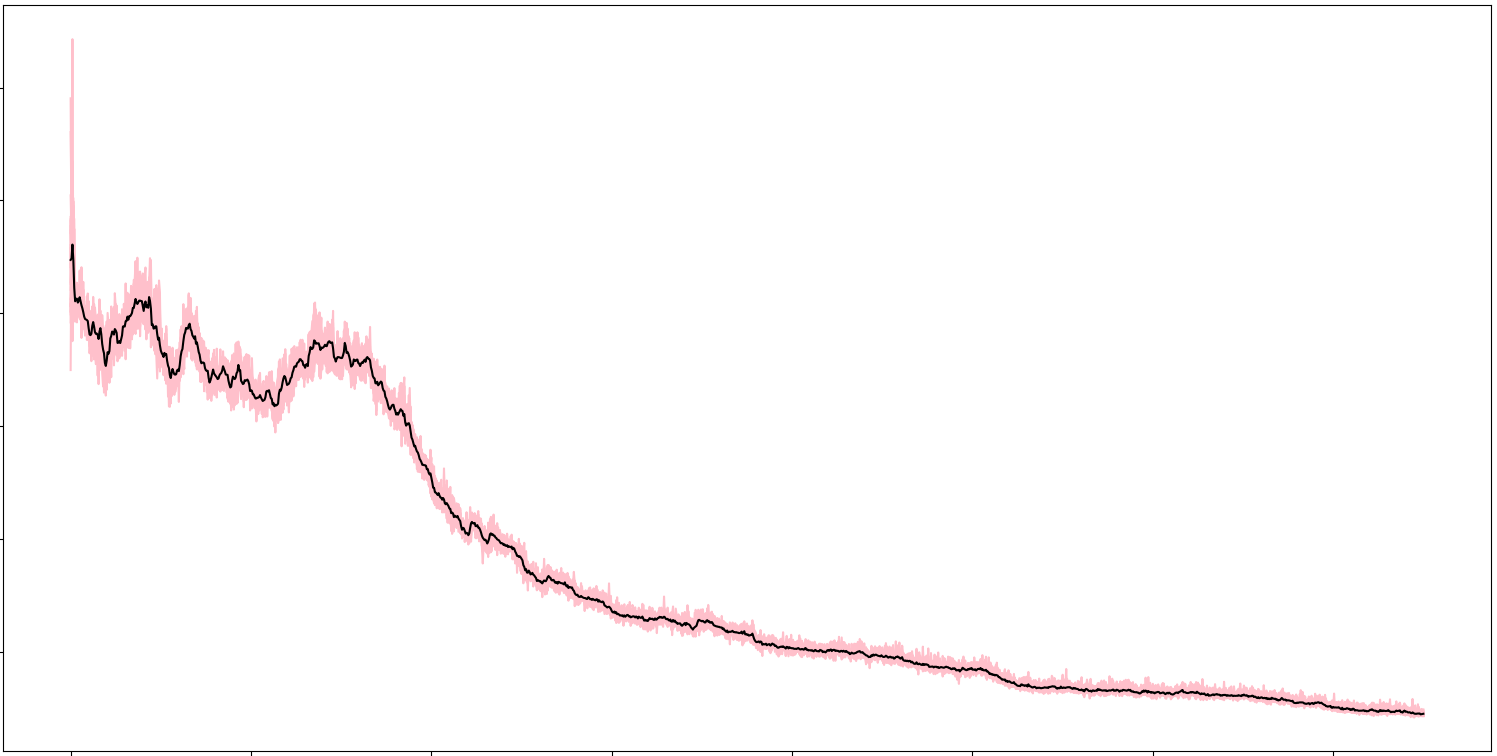
\includegraphics[width=0.35\textwidth]{images/cross_alterniranje.png}} 
    \subfigure[]{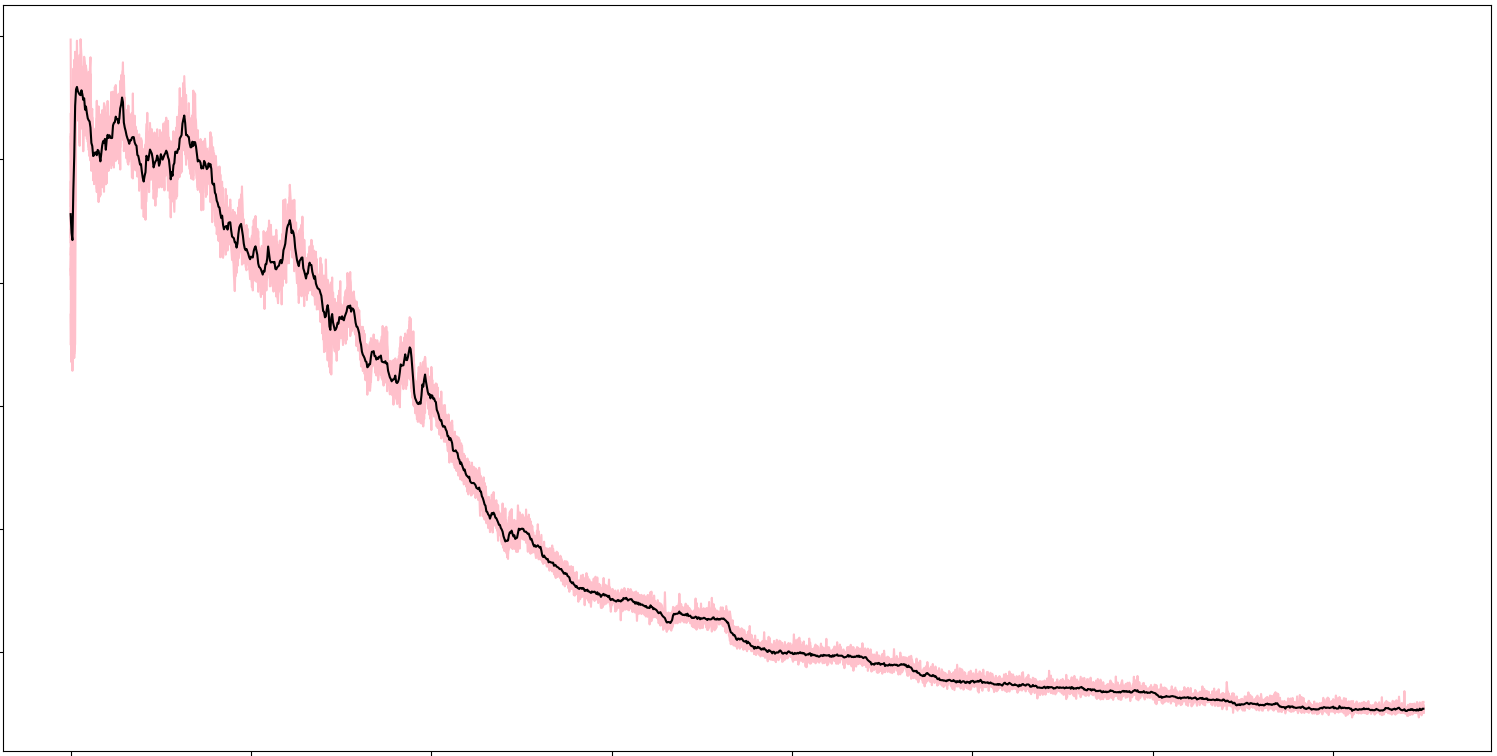
\includegraphics[width=0.35\textwidth]{images/cross_alterniranje3.png}}
    \subfigure[]{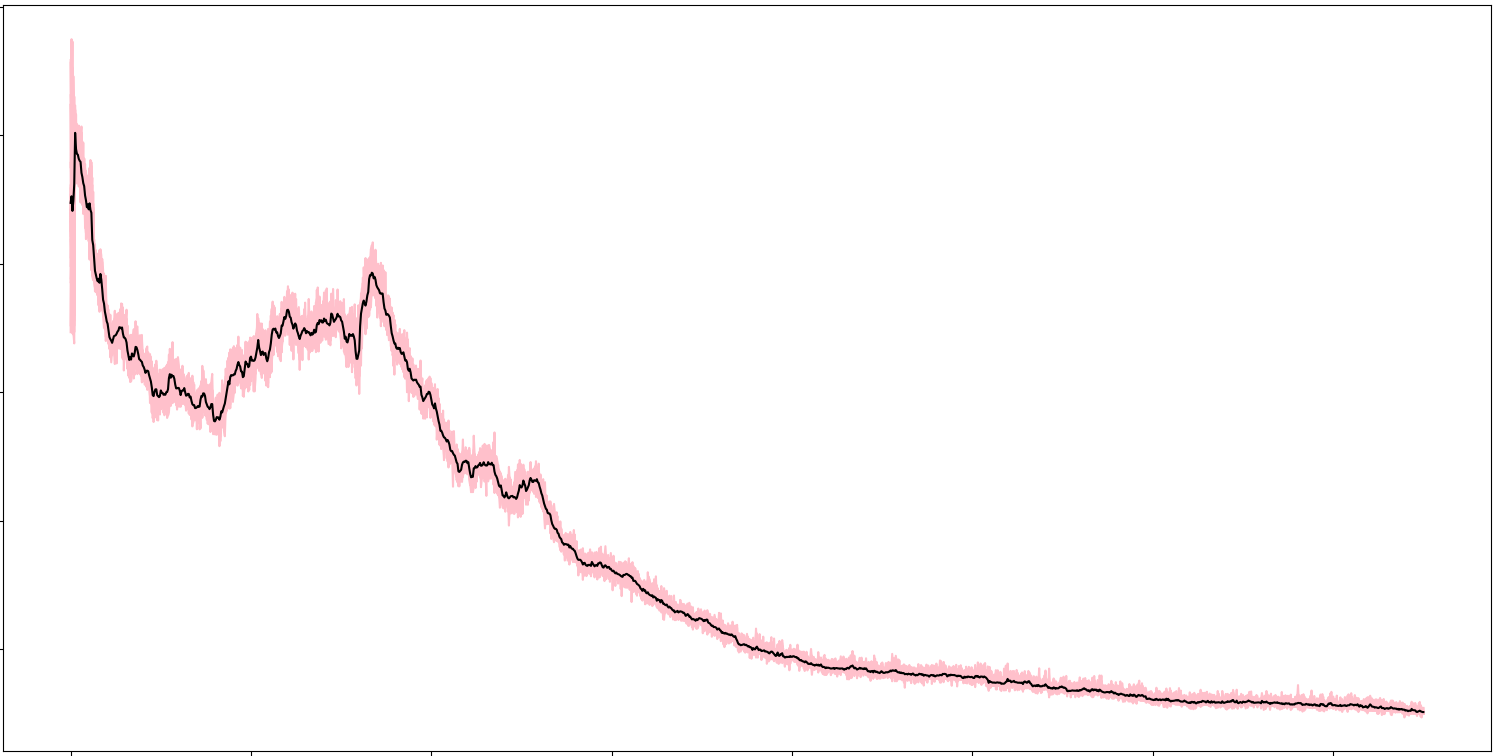
\includegraphics[width=0.35\textwidth]{images/cross_pola.png}}
    \caption{(a) nasumično (b) naizmjenično s K=1 (c) naizmjenično s K=3 (d) pola rasporeda}
    \label{fig:krizanja}
\end{figure}

Sve vrste križanja rasporeda testirane su s 1500 iteracija, razlike su vidljive u početnim iteracijama algoritma, kada svaki operator postiže drugačije rezultate. Nakon već 1000 iteracija, svi operatori djeluju otprilike jednako bez primjetnih razlika. Zbog toga je odabran operator nasumičnog križanja jer može potencijalno pružati jače svojstvo otpora konvergenciji od ostalih zbog komponente nasumičnosti koju sadrži.

\section{Vremenska komponenta i veličina populacije}

Elitizam i operatori križanja ne mijenjaju značajno vrijeme izvođenja. Izračun kazne je konstantan, stoga neovisno o konfiguraciji ima jednak utjecaj. Operator odabira roditelja, veličina populacije i stopa mutacija utječu na vrijeme potrebno za izvršavanje jedne iteracije i pronalazak kvalitetnog rasporeda.

Testiranje vremena izvođenja  testira se na 300 iteracija sa 100 rasporeda u populaciji.

\begin{table}[htb]
\caption{Vrijeme izvođenja ovisno o operatoru odabira roditelja.}
\label{tbl:iter-roditelj}
\centering
\begin{tabular}{lll} \hline
proporcionalna selekcija & proporcionalna selekcija (poboljšana) &  turirska selekcija (K = 3)\\ \hline
13.87 & 14.53 & 15.05\\ \hline
\end{tabular}
\end{table}

Vrijeme izvođenja poboljšane verzije proporcionalne selekcije je veće kao što je očekivano, ali operator turnirske selekcije, iako je sporiji od ostalih, pruža puno bolje rezultate zbog čega se i dalje smatra najboljim operatorom za ovaj zadatak.

Nadalje, s većom stopom mutacije, vrijeme izvođenja algoritma će se povećati jer je potrebno generirati i primijeniti više vrijednosti, no to nije fokus, već brzina konvergencije ovisno o stopi mutacije. Sa stopom mutacije nula, nakon svega nekoliko iteracija učenje prestaje, sa stopom iteracije oko 1\% učenje uspori, ali ne prestaje, a sa stopom oko 0.2\% učenje je najbrže.

\newpage

\begin{figure}[htb]
\centering
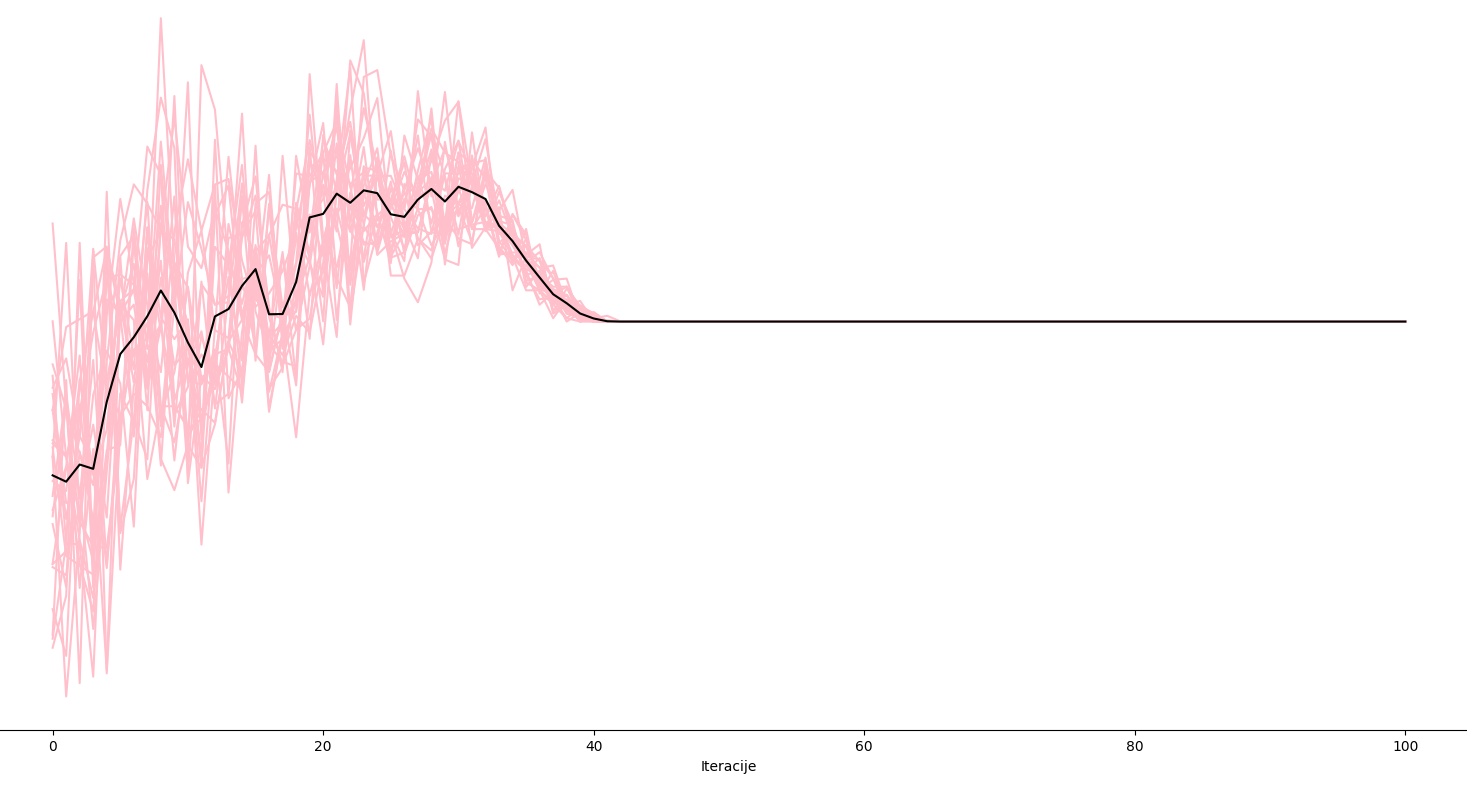
\includegraphics[width=14cm]{images/mutacija_nula.png}
\caption{Mutacija sa stopom mutacije 0.}
\label{fig:mutacija_nula}
\end{figure}

\begin{figure}[htb]
\centering
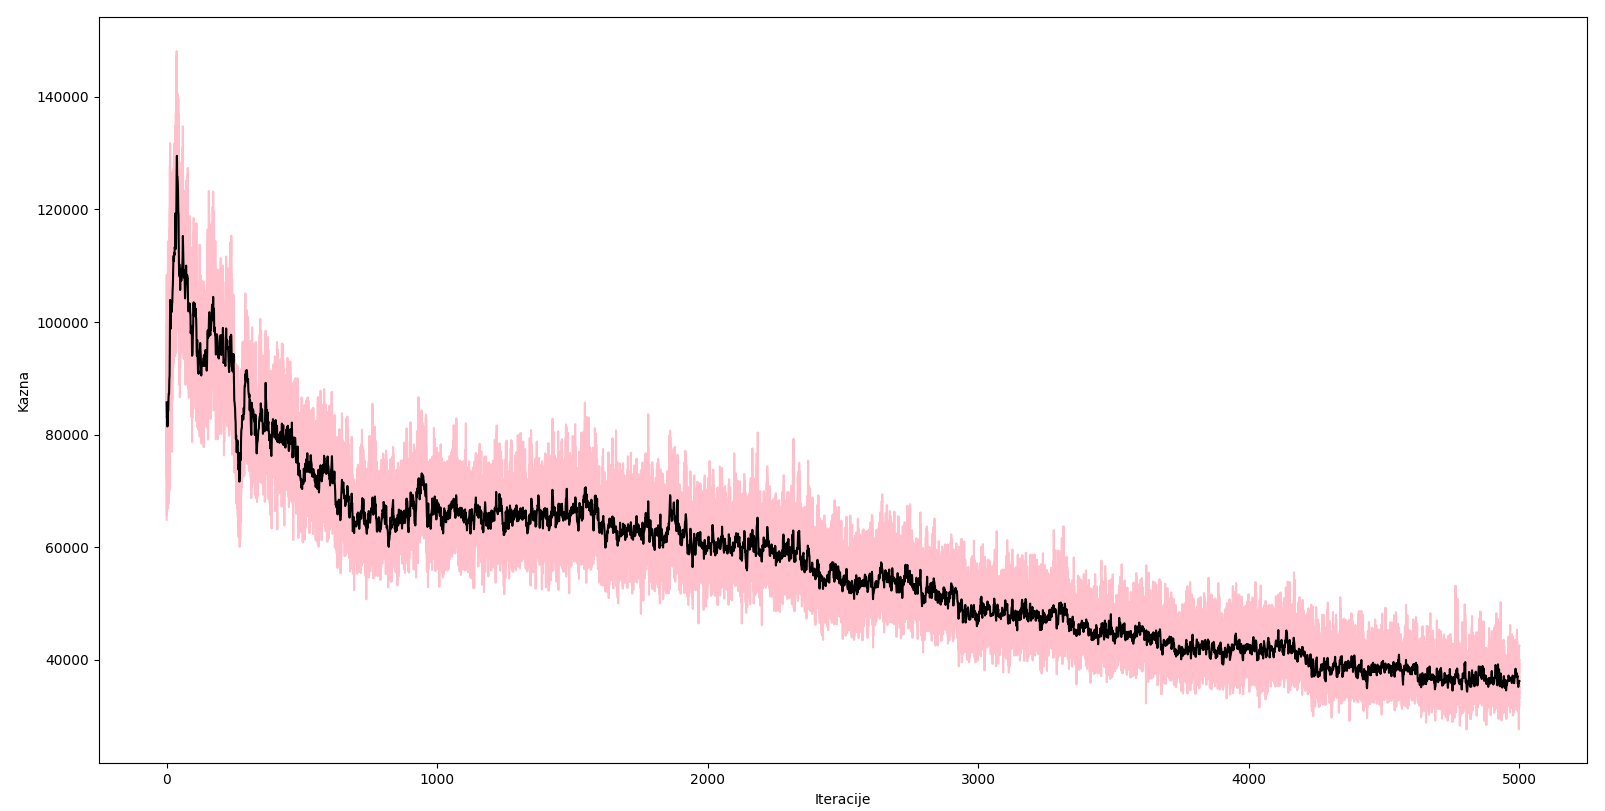
\includegraphics[width=14cm]{images/mutacija_velika.png}
\caption{Mutacija sa stopom mutacije 0.1.}
\label{fig:mutacija_velika}
\end{figure}

S visokom stopom mutacije od 1\% u prosjeku se mijenja termin za 8.3 studenta, zbog toga raspored jako sporo konvergira i generirana djeca su jako različita što je vidljivo na grafu.

Posljednje je preostalo usporediti brzinu pronalaženja rasporeda određene kvalitete. 
\newpage

Uspoređuje se pronalazak rasporeda s kaznom 20000, 1000 i 7500 s populacijom 15, 25, 50, 150 i 250, sva vremena su izražena u sekundama.

\begin{table}[htb]
\caption{Vrijeme izvođenja ovisno o operatoru odabira roditelja.}
\label{tbl:iter-roditelj}
\centering
\begin{tabular}{llll} \hline
populacija/kazna & 20000 &  10000 & 7500\\ \hline
15 & 5.81 & 13.74 & 19.22\\
25 & 8.14 & 10.01 & 15.68\\
50 & 7.69 & 15.52 & 24.39\\
150 & 13.76 & 25.09 & 40.63\\ \hline
\end{tabular}
\end{table}

Iz prikazane tablice vidljivo je kako je upravo 25 najbolja veličina populacije, iako na početku su opcije poput 50 i 15 brže, kasnije u algoritmu je potreban velik broj iteracija kako bi se prošao što veći broj iteracija i opet što veća raznolikost. Za kraj pružam prikaz referentnih pretpostavki, ali uz povećanje broja iteracija na 10000.

\begin{figure}[htb]
\centering
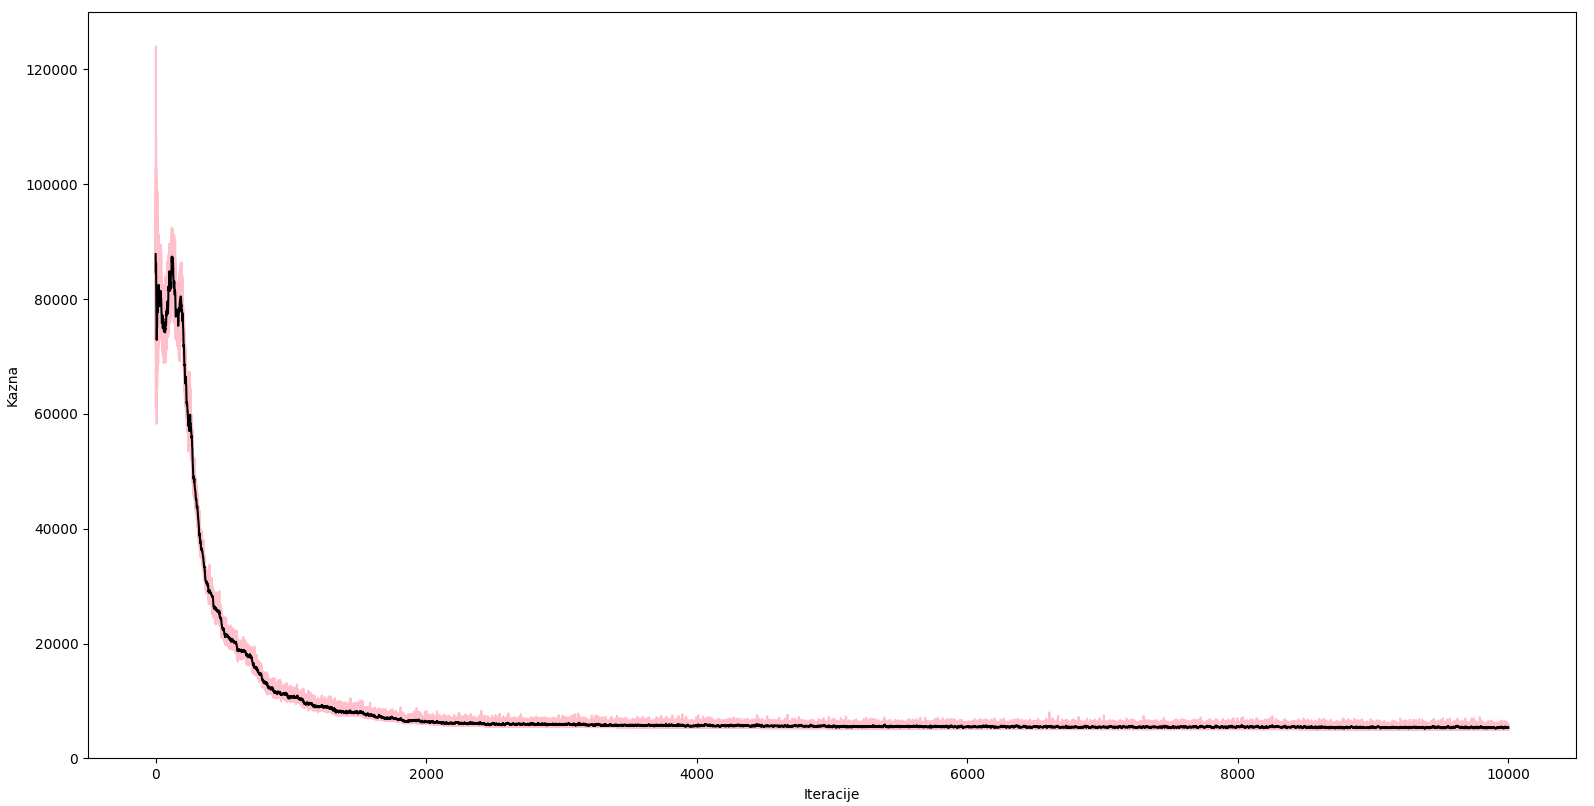
\includegraphics[width=15cm]{images/final.png}
\caption{Referentne postavke algoritma.}
\label{fig:final}
\end{figure}

Nakon 10000 iteracija algoritam je pronašao raspored bez preklapanja i s potrebnim kapacitetima za svaki termin s konačnom kaznom od 5012.

\chapter{Zaključak}

U sklopu ovog rada predstavljen je problem izrade raspodjele studenata u nastavne i ispitne grupe te niz prepreka i ograničenja koja postoje prilikom izrade rasporeda. Problem se svodi na pametnu pretragu velikog prostora stanja.

Jedna od metoda pretrage rješenja je primjena metaheuristike, točnije generacijskog genetskog algoritama gdje se modeliranjem biološkog procesa evolucije simulira proces opstanka najjačih i izumiranja najslabijih jedinki.

Opisan je rad algoritma kao i svih njegovih dijelova. Predložen je prikaz rasporeda u memoriji kao niz studenata s dodijeljenim terminom, takva reprezentacija pruža jednostavan i efikasan zapis. Umjesto izračuna dobrote, predložena je uporaba kazne.

Ispostavilo se kako elitizam pozitivno utječe na dobivene rezultate. Za rasporede je predloženo da se vrednuju prvotno po broju preklapanja, a tek on po kazni. Predloženo je da se kazni pribrajaju broj preklapanja, udaljenost dodijeljenog termina od sljedećeg najbližeg i razlika između dostupnog i iskorištenog kapaciteta učionice.

Kao operator odabira roditelja najbolje se pokazala turnirska selekcija, a za operator križanja nije pronađena bitna razlika, međutim odabran je operator nasumičnog križanja. Za mutaciju je pokazano da je najbolja relativno mala stopa mutacije takva da u prosjeku mutira selekcija za jedan do dva studenta.

Posljednje, populacija od dvadesetak rasporeda pruža najbolja svojstva raznolikosti uz veliku brzinu prolaska kroz velik broj iteracija.

Kao krajnji rezultat ovog rada definirana je konfiguracija algoritma koja u konačnici generira iskoristiv raspored s terminima laboratorijskih vježbi bez preklapanja i s takvim svojstvima koja odgovaraju stunentima.

\bibliography{literatura}.
\bibliographystyle{fer}

\begin{sazetak}
Genetski algoritmi su primjenjivi na širok spektar problema, a izrada rasporeda sati jedan je od konkretnih i primjenjivih problema. U sklopu ovog rada opisan je rad generacijskog genetskog algoritma s mogućim rješenjima raznih operatora potrebnih za rad algoritma. Uspoređeni su utjecaji različitih konfiguracija i rezultata dobivenih iz provedenih eksperimenata kako bi se ispitala kvaliteta generiranih rasporeda. Usporedbom rezultata odabrana je konfiguracija koja je predložena kao konačno rješenje problema.

\kljucnerijeci{Operatori, generacijski, eksperimenti, kvaliteta, konfiguracija.}
\end{sazetak}

\engtitle{Generating a schedule of laboratory exercises using a genetic algorithm}
\begin{abstract}
Genetic algorithms are applicable to a wide range of problems, and class scheduling is one of concrete and applicable problems. As part of this paper, the operation of the generational genetic algorithm is described with the possible solutions of various operators required for the operation of the algorithm. The effects of different configurations and the results obtained from the conducted experiments were compared in order to examine the quality of the generated schedules. By comparing the results, the configuration that was proposed as the final solution to the problem was selected.

\keywords{Operators, generational, experiments, quality, configuration.}
\end{abstract}

\end{document}